\documentclass[leqno,12pt]{article}


\usepackage{ifxetex}

% PAGE SETTINGS %

\parskip 0in
\parindent 0.32in

\usepackage[letterpaper]{geometry}
\geometry{text={5.562306in,9.0in},
headsep=0.5in,footskip=0.5in,centering}


\ifxetex
  \usepackage[T1]{fontenc}
  \usepackage[no-math]{fontspec}

  \setmainfont[Scale=1.0]{Kepler Std Light}

  \usepackage[eucal,mtphrb,mtpfrak,noamssymbols,
  	      subscriptcorrection,zswash]{mtpro2}

  \DeclareMathSizes{12}{12}{9}{7}
\else
  \usepackage[T1]{fontenc}
  \usepackage{lmodern}

  % to match mt2pro
  \usepackage{upgreek}
  \newcommand{\mbf}{\mathbf} 

  \usepackage{mathrsfs}

\fi
  
\usepackage{amssymb}
\usepackage[scr=boondox, scrscaled=1]{mathalfa}


% PACKAGES %

\usepackage{amsmath}
\usepackage{graphicx}
\usepackage{enumitem}
\usepackage{comment}
\usepackage{url}
\usepackage{marginnote}
\usepackage{booktabs}
\usepackage{bm}
\usepackage{mdframed}
\usepackage{xfrac}


% ALGORITHMS %

\usepackage{float}
\floatstyle{ruled}
\newfloat{algorithm}{hpt}{lop}
\floatname{algorithm}{Algorithm}

% THEOREMS %

\usepackage{amsthm}
\newtheoremstyle{mytheoremstyle}
{\topsep}                    % Space above
{\topsep}                    % Space below
{\slshape}                   % Body font
{0.32in}                           % Indent amount
{\bfseries}                  % Theorem head font
{.}                          % Punctuation after theorem head
{0.08in}                       % Space after theorem head
{}  % Theorem head spec (can be left empty, meaning ‘normal’)

\theoremstyle{mytheoremstyle}

\makeatletter
\@ifclassloaded{report}{
   \newtheorem{theorem}{Theorem} }
{  \newtheorem{theorem}{Theorem}[section] }
\makeatother


\newtheorem{thm}[theorem]{Theorem}
\newtheorem{proposition}[theorem]{Proposition}
\newtheorem{lemma}[theorem]{Lemma}
\newtheorem{corollary}[theorem]{Corollary}
\newtheorem{definition}[theorem]{Definition}
\newtheorem{remark}[theorem]{Remark}
\newtheorem{example}[theorem]{Example}
\newtheorem{condition}[theorem]{Condition}
\newtheorem{assumption}[theorem]{Assumption}
\newtheorem{claim}[theorem]{Claim}

\newtheorem*{theo}{Theorem}
\newtheorem*{lemm}{Lemma}
\newtheorem*{defn}{Definition}
\newtheorem*{prop}{Proposition}
\newtheorem*{assm}{Assumption}
\newtheorem*{cond}{Condition}
\newtheorem*{coro}{Corollary}
\newtheorem*{remk}{Remark}
\newtheorem*{expl}{Example}
\newtheorem*{clai}{Claim}

\renewcommand\qedsymbol{$\blacksquare$}
\renewenvironment{proof}[1][\proofname]{{\scshape #1. }}
{\qed\vspace{0.16in}}

% SECTIONS %
\usepackage{titlesec}

% section that begins a paragraph (. separator)
\titleformat{\section}[hang]
{\centering\bfseries}
{\thesection.}{0.04in}{}[]
\titlespacing{\section}{0.32in}{0.32in}{0.08in}

\titleformat{\subsection}[runin]
{\bfseries} 
{\thesubsection.}{0.04in}{}[.]
\titlespacing{\subsection}{0.32in}{0.08in}{0.08in}

% ABSTRACT

\renewcommand{\abstractname}{\bf Abstract}

\renewenvironment{abstract}
{\small
\begin{center}
  \bfseries \abstractname\vspace{0in}\vspace{0pt}
\end{center}
\list{}{
	\setlength{\leftmargin}{0.5in}
    \setlength{\rightmargin}{\leftmargin}
	\itemindent \parindent} 
  \item\relax}
{\endlist}


% TABLES AND FIGURES

\usepackage{caption}
\captionsetup[figure]{margin=0.16in,
	labelsep=period,labelfont=bf,textfont=it}
\captionsetup[table]{margin=0.16in,
	labelsep=period,labelfont=bf,textfont=it}


% REFERENCES %

\usepackage{hyperref}
\hypersetup{colorlinks=true, allcolors=deluge}

\usepackage{harvard}
\makeatletter
\@ifpackageloaded{harvard}{}
  {\newcommand{\citeasnoun}{\cite}}
\makeatother

\newcommand{\ci}{\citeasnoun}
\newcommand{\req}[1]{(\ref{#1})}

\newcommand{\hci}[2]{ \href{#2}{\ci{#1}} }
\newcommand{\hcite}[2]{ \href{#2}{\cite{#1}} }


% FRAMES %

\global\mdfdefinestyle{clean}{%
linecolor=black,linewidth=0.5pt,%
leftmargin=0.32in,rightmargin=0.32in
}

\global\mdfdefinestyle{wide}{%
linecolor=black,linewidth=0.5pt,%
leftmargin=0in,rightmargin=0in
}









%\newif\ifhide
%\hidetrue %\hidefalse
%\newcommand{\hide}[1]{\ifhide {} \else {#1} \fi} 





% SPACING/TEXT %

\newcommand{\s}[1][1]{\hspace{#1pt}}
\newcommand{\mst}{{\scalebox{0.6}[0.6]{\(\hspace{-1pt}{*}\)}}}

\newcommand{\tq}[1]{{\textquotedblleft #1\textquotedblright}}
\newcommand{\ts}[2]{{#1\textsubscript{#2}}}


% PROBABILITY %

\newcommand{\cid}{\overset{\scrD}{\rightarrow}}
\newcommand{\eqd}{\overset{\scrD}{=}}
\newcommand{\cip}{\overset{p}{\rightarrow}}
\newcommand{\cas}{\overset{a.s.}{\rightarrow}}
\newcommand{\sip}{\overset{p}{\sim}}
\newcommand{\sas}{\overset{a.s.}{\sim}}

\newcommand{\setst}{\mathbb} % set style
\newcommand{\oprst}{\textup} % operator style

\newcommand{\inds}[1]{ \mathbb{1}_{ \s[-0.5] {#1} }}
\newcommand{\indf}[1]{ \mathbb{1}_{ \s[-0.5] \{#1\} }}

\newcommand{\ms}{\scalebox{0.66}[1.0]{\( - \)}}

\newcommand{\var}{\oprst{var}}
\newcommand{\std}{\oprst{std}}
\newcommand{\cov}{\oprst{cov}}
\newcommand{\Var}{\oprst{Var}}
\newcommand{\Cov}{\oprst{Cov}}
\newcommand{\Std}{\oprst{SD}}
\newcommand{\MSE}{\oprst{MSE}}
\newcommand{\RMSE}{\oprst{RMSE} }
\newcommand{\Exp}{\oprst{E}\s[.5]}
\newcommand{\Prb}{\oprst{P}\s[.5]}
\newcommand{\Qrb}{\ensuremath{\oprst{Q}\s[.5]}}

\newcommand{\tsum}{{\textstyle\sum\nolimits}}

% SETS / MATH $

\newcommand{\nn}{\bbN}
\newcommand{\rn}{\bbR}
\newcommand{\zn}{\bbZ}
\newcommand{\qn}{\bbQ}

\newcommand{\Img}{\mathrm{Im}}
\newcommand{\Rea}{\mathrm{Re}}
\newcommand{\im}{\mathrm{i}}


\newcommand{\bst}{ \s[1.5] | \s[1.5] }
\newcommand{\cst}{ \s[0.5] : \s[0.5] }
\newcommand{\sst}{ \s[2.0] ; \s[0.5] }


\newcommand{\mat}[1]{\mbf{#1}}
\newcommand{\ones}{\rme}
\newcommand{\tr}{\textrm{tr}}   
\newcommand{\diag}{\textrm{diag}}   

% LETTER STYLES %
\usepackage{pgffor}

\foreach \x in {A,B,...,Z,a,b,...,z} 
{
  \expandafter\xdef\csname cal\x\endcsname{\noexpand 
	\ensuremath{\noexpand\mathcal{\x}}}
  \expandafter\xdef\csname scr\x\endcsname{\noexpand 
	\ensuremath{\noexpand\mathscr{\x}}}
  \expandafter\xdef\csname bb\x\endcsname{\noexpand 
	\ensuremath{\noexpand\mathbb{\x}}}
  \expandafter\xdef\csname rm\x\endcsname{\noexpand 
	\ensuremath{\noexpand\mathrm{\x}}}
  \expandafter\xdef\csname bf\x\endcsname{\noexpand 
	\ensuremath{\noexpand\mbf{\x}}}
}


% GREEK %

\newcommand{\ep}{\epsilon}


% ARROWS %

\newcommand{\upto}{ \uparrow }
\newcommand{\downto}{ \downarrow }
\newcommand{\nto}{ \nrightarrow }



% COLABORATION %

\newcommand{\astext}[1]{\delugetext{#1 -- alex}}
\newcommand{\mvtext}[1]{\delugetext{#1 -- matt}}

% LOCAL %

\newcommand{\Rcll}{C\`adl\`ag }
\newcommand{\rcll}{c\`adl\`ag }

\newcommand{\prj}[2]{\langle #1 , #2 \rangle}

\newcommand{\ip}[2]{\langle #1 , #2 \rangle}

\newcommand{\cv}{\rmd}
\newcommand{\av}{\upmu}

\newcommand{\sv}{\updelta}
\newcommand{\fv}{\upvarsigma}






\usepackage{color}
\usepackage[table]{xcolor}

\definecolor{red}{rgb}{1,0,0}
\definecolor{gray}{rgb}{0.5,0.5,0.5}
\definecolor{darkgray}{rgb}{0.4,0.4,0.4}
\definecolor{blue}{rgb}{0,0,1}
\definecolor{green}{rgb}{0,1,0}
\def\graytext#1{{\color{gray}{{#1}}\color{gray}}}
\def\darkgraytext#1{{\color{darkgray}{{#1}}\color{darkgray}}}
\def\redtext#1{{\color{red}{{#1}}\color{red}}}
\def\bluetext#1{{\color{blue}{{#1}}\color{blue}}}
\def\greentext#1{{\color{green}{{#1}}\color{green}}}


\definecolor{deluge}{RGB}{124, 113, 173}
\definecolor{bamboo}{RGB}{220, 92, 5}
\definecolor{yellow}{RGB}{255, 172, 0}
\definecolor{orange}{RGB}{255, 144, 0}
\definecolor{oyster}{RGB}{151, 139, 125}
\definecolor{coral}{RGB}{199, 186, 167}
\definecolor{downy}{RGB}{110, 197, 184}

\def\delugetext#1{{\color{deluge}{{#1}}\color{deluge}}}
\def\bambootext#1{{\color{bamboo}{{#1}}\color{bamboo}}}
\def\yellowtext#1{{\color{yellow}{{#1}}\color{yellow}}}
\def\orangetext#1{{\color{orange}{{#1}}\color{orange}}}
\def\oystertext#1{{\color{oyster}{{#1}}\color{oyster}}}
\def\coraltext#1{{\color{coral}{{#1}}\color{coral}}}
\def\downytext#1{{\color{downy}{{#1}}\color{downy}}}




\usepackage{setspace}
\usepackage{pgfornament}

\newcommand{\secbreak}{\begin{center}
\vspace{0.16in}\pgfornament[width=2in]{88}
\end{center}}

% for bold sum and product below
\usepackage{bm}

\newcolumntype{C}[1]{>{\centering\let\newline\\
	\arraybackslash\hspace{0pt}}m{#1}}
\newcolumntype{L}[1]{>{\raggedright\let\newline\\
	\arraybackslash\hspace{0pt}}m{#1}}

\renewcommand{\baselinestretch}{1.16} 

\begin{document}

% enable bold sum and product in xetex
\ifxetex
  \let\lsum\sum
  \renewcommand{\sum}{\bm{\lsum}}

  \let\lprod\prod
  \renewcommand{\prod}{\bm{\lprod}}
\else
\fi

\newcommand{\upep}{\upepsilon}
\newcommand{\mv}{\sigma_\rmM}
\newcommand{\mb}{\beta^{\rmM}}

{\setstretch{1.0}
\noindent
{\bf Asset model analytics v1.1}
\noindent
\hfill {\today} \noindent
\rule{\textwidth}{0.01in}


\section{Model analytics}

For the general statisfical model of asset return 
(see \verb|am_standards|) given by
\begin{align}
  y = f(\psi) + \upepsilon \s .
\end{align}
we define a series of analyses that inform financial modeling,
interpretability, statistical estimation, hypothesis testing 
and performance evaluation.

The covariance matrix plays a primary role in the 
distibution of asset return:
\begin{align}
  \Var(y) = \Sigma \s .
\end{align}
In practice, we analyze the estimated covariance matrix
$\hat{\Sigma}$, but here we use $\Sigma$ for simplicity.
An asset model typically assumes some particular structure
for $\Sigma$ that suggests particular analyses to perform.
We motivate different types of analyses for the various
models in \verb|am_standards|. (Coversions between the
various models is often possible).

\section{Analytics prototypes}

\begin{verbatim}
 
Input: model with attributes
-- attribute : type (factor, graphical, etc)
-- attribute : estimation_window (start_date, end_data, freq)
-- attribute : method (pca, mtfa, glasso, etc)

Analytics for type = factor:
-- compute_signal -- arg : factor_id 
-- compute_noise
-- compute_size
-- compute_snr
-- compute_skew
-- compute_meltup
-- compute_correlation
-- compute_entropy

\end{verbatim}

\section{Factor model analytics}

Consider the {\bf canonical factor model} for which the covariance has the form
\begin{align}
 \Sigma = \Pi \Psi \Pi^\top +  \Omega
\end{align}
with a diagonal, $q \times q$ postive definite matrix $\Psi$ 
and a full rank $p \times q$ matrix $\Pi$ with othogonal 
columns $\uppi_1, \dots, \uppi_q$ (i.e., 
$\ip{\uppi^k}{\uppi^\ell} = 0$ for all $k \neq
\ell$),\footnote{The inner product could be a weighted one
but here we continue with the standard inner product.}
and a symmertic positive definite matrix $\Omega$ with 
bounded eigenvalues (in dimension $p$).

It is important to undertand the evolution, over time, of 
both components in the decomposition of $\Sigma$ above.
In practice, some estimation procedure (e.g. PCA,
see \verb|pca|), will 
produce estimates of the triplet $(\Pi, \Psi, \Omega)$ which
conforms to the standards in \verb|am_standards|. The following
analytics help study the structure of $(\Pi, \Psi, \Omega)$

The systematic risk component of the canonical factor model
may be written as
\begin{align}
   \Pi \Psi \Pi^\top = 
  \upsigma_{1}^2 \uppi^1 (\uppi^1)^\top 
  + \cdots + \upsigma^2_{q} \uppi^q (\uppi^q)^\top 
\end{align}
and we take $\upsigma^2 \uppi \uppi
= (\upsigma \uppi)(\upsigma \uppi)^\top$ as a representative term
letting $\eta = \upsigma \uppi \in \bbR^p$ which represents the product
of the factor volatility $\upsigma$ times the factor exposures 
$\uppi$. In practice, there is no way to estimate the 
$\upsigma$ and $\uppi$ separately, and we can write
\begin{align}
  \eta \eta^\top = \rmc^2 \s \Big( \frac{\eta}{\rmc} \Big)
   \Big(\frac{\eta}{\rmc} \Big)^\top
\end{align}
for any $\rmc \neq 0$ so that the variance is now identified
as $\upsigma^2 = \rmc^2$ while $\uppi = \frac{\eta}{\rmc}$.



This motivates the analysis of the structure of the 
vector $\eta$ to determine how to best model the individual
components $\upsigma$ and $\uppi$ among other concerns.


\begin{mdframed}[style=clean]
  Let $\eta = \upsigma \uppi \in \bbR^p$, the product of the 
factor volatility and exposure. We are interested in the 
evolution over time of the following quantities.
\begin{itemize}
  \item[--] {\bf Signal.} Denoted by $\rmm(\eta)$ and 
defined by
\begin{align}
  \rmm(\eta) = \tsum_{i=1}^p \eta_i/p \ge 0
\end{align}
where we flip the sign of $\eta$ to ensure nonnegativity.
  \item[--] {\bf Noise.} Denoted by $\rms(\eta)$
and defined by 
\begin{align}
\rms(\eta) = \sqrt{\tsum_{i=1}^p 
(\eta_i-\rmm(\eta))^2/p} \s .
\end{align}
\item[--] {\bf Exposure SNR.} A signal-to-noise ratio defined by
\begin{align}
  \text{SNR}(\eta) = \frac{\rmm(\eta)}{\rms(\eta)} \s .
\end{align}
  \item[--] {\bf Size.} Denoted by $\rmz(\eta)$ and defined
as a scaled length
\begin{align}
  \rmz(\eta) = |\eta|/\sqrt{p} = \sqrt{\ip{(\eta)}{\eta}/p}
  = \sqrt{\rmm^2(\eta) + \rms^2(\eta)} \s .
\end{align}
\item[--] {\bf Skewness.} Denoted by $\rmk(\eta)$ and 
defined as
\begin{align}
 \rmk(\eta) = \frac{\tsum_{i=1}^p (\eta_i - \rmm(\eta))^3/p}
 {\rms^3(\eta) }
\end{align}
\item[--] {\bf Meltup.} Denoted by $\rmu(\eta)$ and 
defined as
\begin{align}
   \rmu(\eta) = \tsum_{i=1}^p \text{sgn}(\eta_i)/p
\end{align}
\item[--] {\bf Correlation.} Denoted by $\rho(\eta)$ and 
defined as
\begin{align}
   \rho(\eta) = \tsum_{i\neq j} \eta_i \eta_j/(p^2-p)
\end{align}
\item[--] {\bf Entropy.}
Denoted by $\rmH(\eta)$ and defined as
\begin{align}  
   \rmH(\eta) = -\tsum_{i=1}^p \rmp_i(\eta) \log \rmp_i(\eta)
\end{align}
for $\rmp_i(\eta) = \upphi(\eta)$ for some probability
density $\upphi$ (e.g. normal).
\end{itemize} 
\end{mdframed}

In particular, the size, signal and noise can all serve
as a proxy for the factor variance, i.e., (one exception
is when the signal $\rmm(\eta)$ is close or equal to zero)
\begin{align}
  \eta \eta^\top 
  &= \rmz^2(\eta) \Big( \frac{\eta}{\rmz(\eta)}
   \frac{\eta^\top}{\rmz(\eta)} \Big)
  = \rms^2(\eta) \Big( \frac{\eta}{\rms(\eta)}
   \frac{\eta^\top}{\rms(\eta)} \Big)
  = \rmm^2(\eta) \Big( \frac{\eta}{\rmm(\eta)}
   \frac{\eta^\top}{\rmm(\eta)} \Big) \\
  &= \upsigma^2 \uppi \uppi^\top \s . \notag
\end{align}
identifying the $\upsigma^2$ with different quantities.


\newpage

\subsection{SSIM estimation}
An SSIM estimate takes the form
\begin{align} \label{estmod}
  \hat{\Sigma} = v^2 h h^\top + \rmD
\hspace{0.16in}
\text{where}
\hspace{0.16in}
\tsum_i h_i \ge 0, 
\hspace{0.16in}
|h| = 1.
\end{align}
There is no way in general to estimate the \tq{sizes} of 
$v \in (0,\infty)$ and $h \in \bbR^p$ so a normalization such as $|h| =1$
has to be selected. Alternatively we can take any,
\begin{align} \label{estnmod}
  \hat{\Sigma} = \Big(\frac{v^2}{Z^2}\Big)
 \eta \eta^\top + \rmD
\hspace{0.16in}
\text{where}
\hspace{0.16in}
\tsum_i \eta_i \ge 0, 
\hspace{0.16in}
|\eta| = Z.
\end{align}
A useful example would set $Z$ equal to the average
entry of $h$ (hence, $\eta$ has unit mean).


Given a $p \times n$ return matrix $\rmY$ ($n$ observations
of $y \in \bbR^p$) we take the sample covariance
and correlation matrices
\begin{align}
 \rmS = \rmY \rmY^\top /n 
  \hspace{0.32in}
 \rmC = \rmV^{-1/2} \rmS \rmV^{-1/2}
  \hspace{0.32in}
  \rmV = \diag(\rmS).
\end{align}
Then we have the following models.
\begin{itemize}
  \item[--] The PCA covariance model takes $h$ to be the 
eigenvector of $\rmS$ with largest eigenvalue $\scrs^2_1$ and 
sets $v^2 = \scrs^2_1$. Further,
$\rmD = \diag(\rmS - v^2 h h^\top)$.
\item[--] The PCA correlation model takes $h$ to be the 
eigenvector of $\rmC$ with largest eigenvalue $\scrc^2_1$ but
sets $v^2 = \scrs^2_1$ (any identity for $\scrs$ and $\scrc$?)
and $\rmD$ as above.
\item[--] James-Stein PCA variation
\item[--] MTFA
\item[--] Graphical model.
\end{itemize}


\section{Beta financial indicators} These can use
the raw beta $\beta$ or the market-cap beta 
$\mb = \rmV^{-1/2} \beta$. The latter is more robust and 
theoretically consistent. It has
\begin{align}
  \mb_i \propto \sqrt{\frac{\beta^2_i}{\mv^2 \beta_i^2 + 
  \updelta_i^2}}
\end{align}
in a strict single index model (SSIM).

\begin{itemize}
  \item[--] {\bf Mean beta.}
 \[ \rmm(\beta) = \sum_{i=1}^p \beta_i /p \]
  \item[--] {\bf Beta dispersion.}
   \[ \rmd^2(\beta) = \rms^2(\beta)/\rmm^2(\beta) \]
  where 
$\rms^2(\beta) = \sum_{i=1}^p (\beta^2_i 
  -\upmu(\beta))^2/p$.
  \item[--] {\bf Beta skewness.}
  \[ \rmk(\beta) = \rmm_3(\beta)/\rms^2(\beta) \]
  where $\rmm_3(\beta) = \sum_{i=1}^p 
  (\beta_i - \upmu(\beta))^3/p$.
  \item[--] {\bf Melt up.} (number positive minus number negative beta).
   \[ \rmM (\beta) = \sum_{i=1}^p \text{sign}(\beta_i) /p \]
  \item[--] {\bf Average pairwise correlation.} For a covariance
matrix $\Sigma = (\Sigma_{ij})$,
 \[ \rho(\Sigma) = \sum_{i\neq j} \frac{\Sigma_{ij}}
{\sqrt{\Sigma_{ii}\Sigma_{jj}}}/(p^2-p) \]
We can also define the average pairwise correlation of Beta
(or any factor $\beta$) as
  \[ \rho(\beta) = \sum_{i\neq j} \beta_i \beta_j
   / (p^2-p) \]
which is rougly $\upmu^2(\beta)$ for $p$ large.
Note that in a SSIM, \[ \rho(\mb) = \rho(\Sigma)\s . \]
 \item[--] {\bf Entropy.} Let $\phi$ be some probability density
(e.g.. normal). 
Let $\rmp_i(\beta) = \phi(\beta_i)$.
  \[ \rmH(\beta) = -\sum_{i=1}^p \rmp_i(\beta) 
\log (\rmp_i(\beta)) \]
\end{itemize}

\section{Nonbeta financial indicators}
Portfolio variances.

\begin{itemize}
\item[--] {\bf Market volatility.} This is simply $\mv$ in
model $\req{model}$. In the estimated model this may be taken
as $v$ in $\req{estmod}$, or for the version of $\req{estnmod}$
that assumes a unit-mean beta,
\begin{align}
   v \rmm(h) \s .
\end{align}
\item[--] {\bf Portfolio volatility.} For a portfolio
$w$ computed based on covariance $\Sigma$,
\[
 \sqrt{w^\top  \Sigma w}
\]
is the volatility of $w$. Similarly for an estimated 
$\hat{w}$ based on $\hat{\Sigma}$ (i.e.,
$\sqrt{\hat{w}^\top  \Sigma \hat{w}}$)
. Then,
\[
 \sqrt{\hat{w}^\top  \Sigma \hat{w}}
\]
is the realized portfolio variance. (When $\Sigma$ is 
not available an out-of-sample estimate may be used).
\item[--] {\bf Diversification index.} For a portfolio
$w$ the following (Herfindahl) index measures diversification
(variations are typically norms $|| \cdot ||$ of $w$),
\[ \rmH\rmI(w) = \sum_{i=1}^p w_i^2 \s .
\]
\end{itemize}

A portfolio based purely on $\Sigma$ (or $\hat{\Sigma}$)
is the one with minimum variance, i.e.,
\begin{equation}
\begin{aligned}
  \min_w \s[2] &w^\top \Sigma w \\
 \text{s.t. }  &w^\top \rme = 1 \\
      &(w \ge 0)
\end{aligned}
\end{equation}
for $\rme = (1,\dots, 1)^\top$ and
with the no short sales constraint ($w \ge 0$) optional.

The solution may be stated explitly in the SSIM $\Sigma
= \mv^2 \beta \beta^\top + \Delta$.
\[  w = 
\frac{\Delta^{-1} (\rme - \theta \beta)}
{\rme^\top \Delta^{-1} (\rme - \theta \beta)}
\]
where $\theta$ for the portolio allowing short sales is
\begin{align}
 \theta = \frac{ \sum_{i=1}^p \beta_i/\delta_i^2}
{1/\mv^2 +  \sum_{i=1}^p \beta^2_i/\delta_i^2}
\end{align}
and we replace $\sum_{i=1}^p$ with $\sum_{\theta\beta_i <1}$
to obtain the solution with no short sales.


\begin{figure}[htp]
\begin{center}
  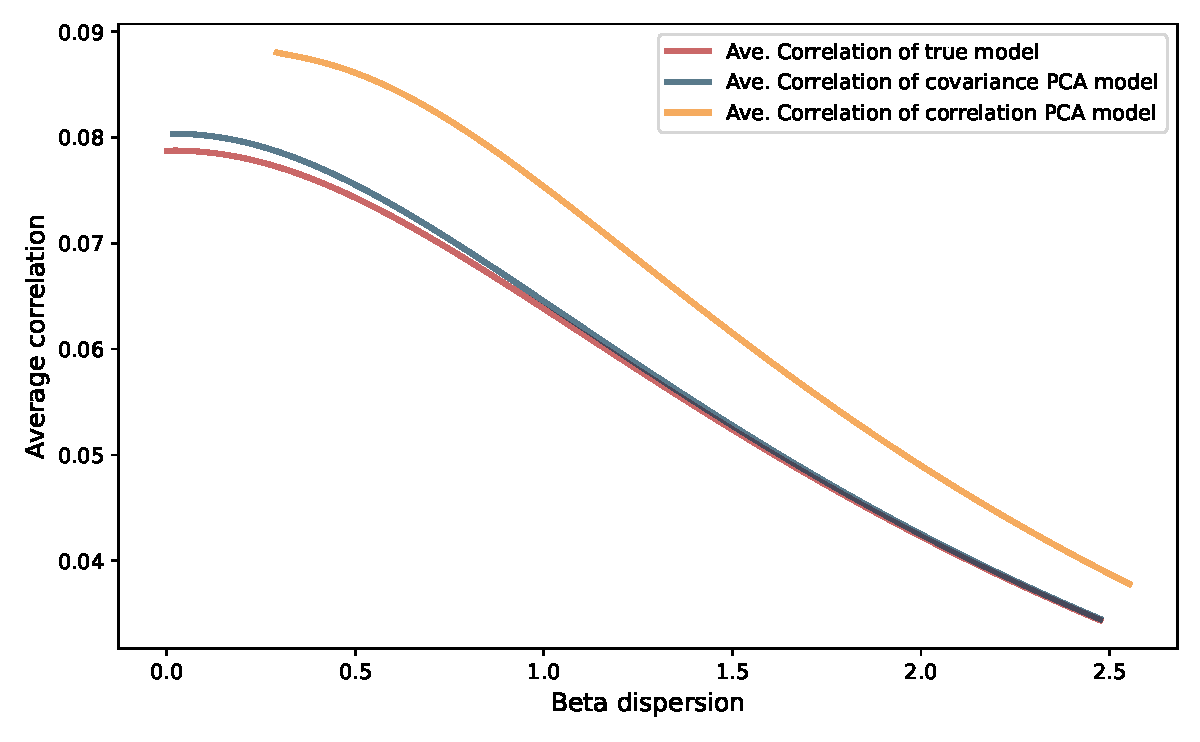
\includegraphics[scale=0.33]{img/DispersionvsCorrelation1factorsN512T256fvol16minsvol30maxsvol90}
  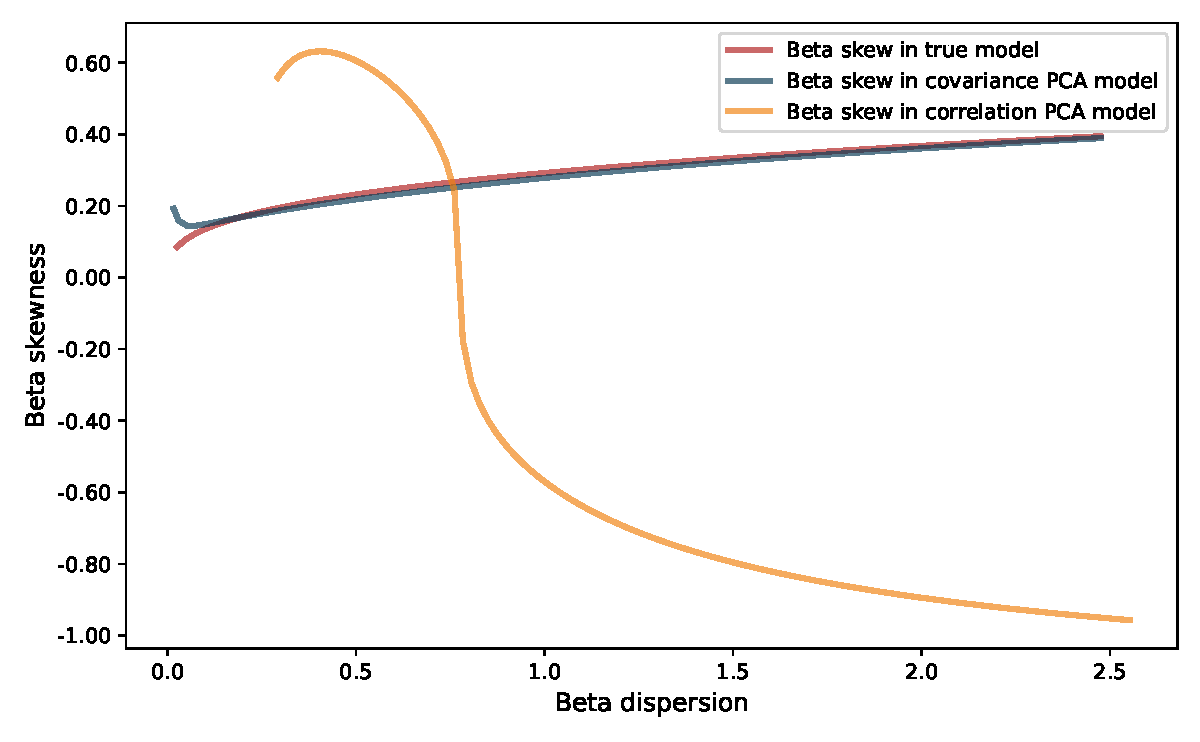
\includegraphics[scale=0.33]{img/DispersionvsSkew1factorsN512T256fvol16minsvol30maxsvol90}
  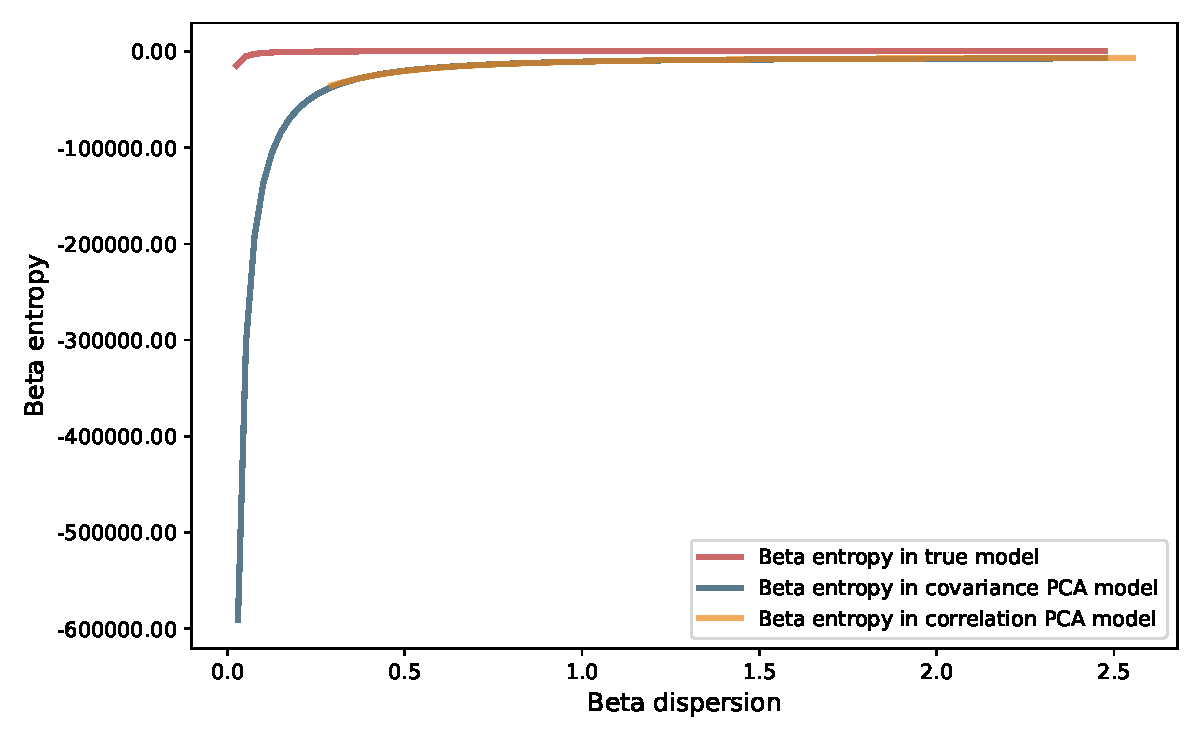
\includegraphics[scale=0.33]{img/DispersionvsEntropy1factorsN512T256fvol16minsvol30maxsvol90}
  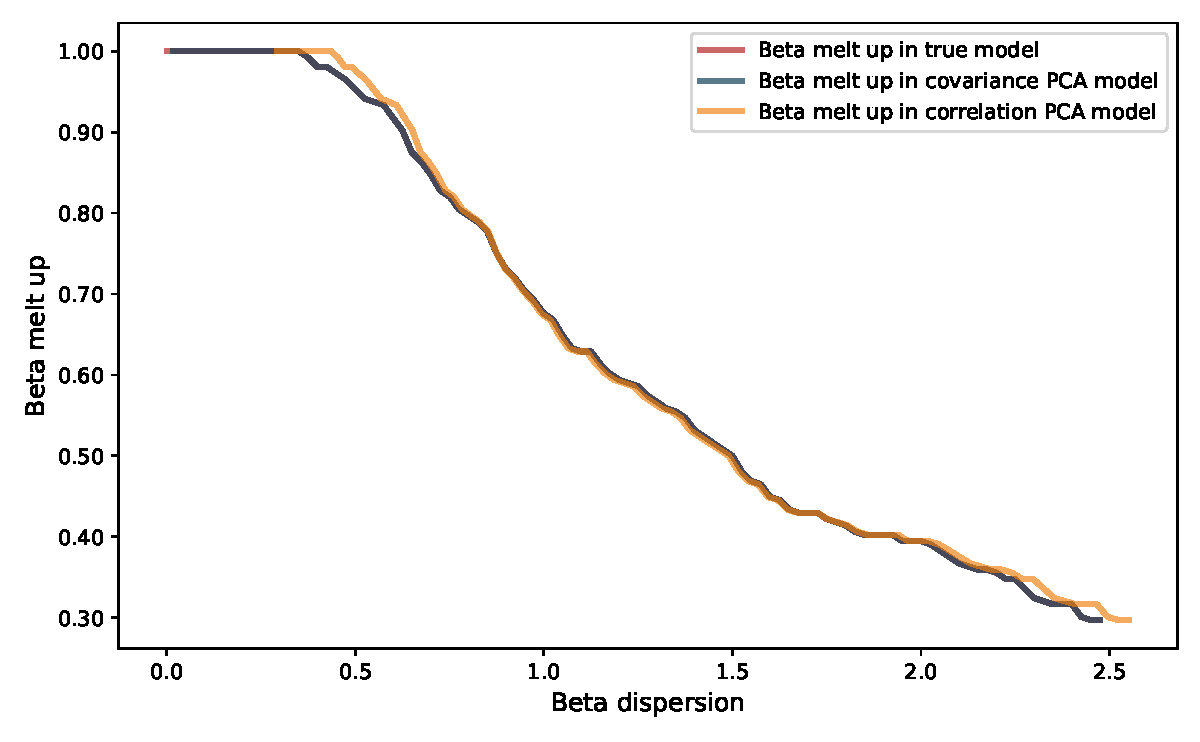
\includegraphics[scale=0.33]{img/DispersionvsMeltup1factorsN512T256fvol16minsvol30maxsvol90}
  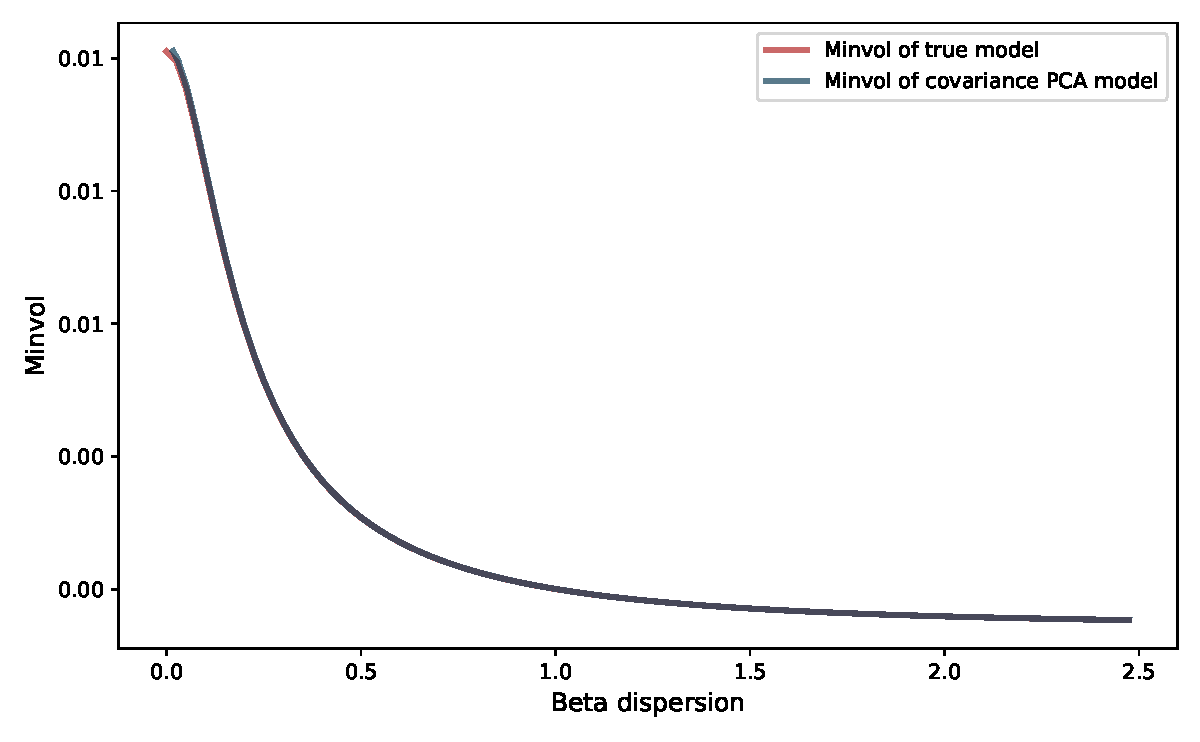
\includegraphics[scale=0.33]{img/DispersionvsPortfolioLSMinvol1factorsN512T256fvol16minsvol30maxsvol90}
  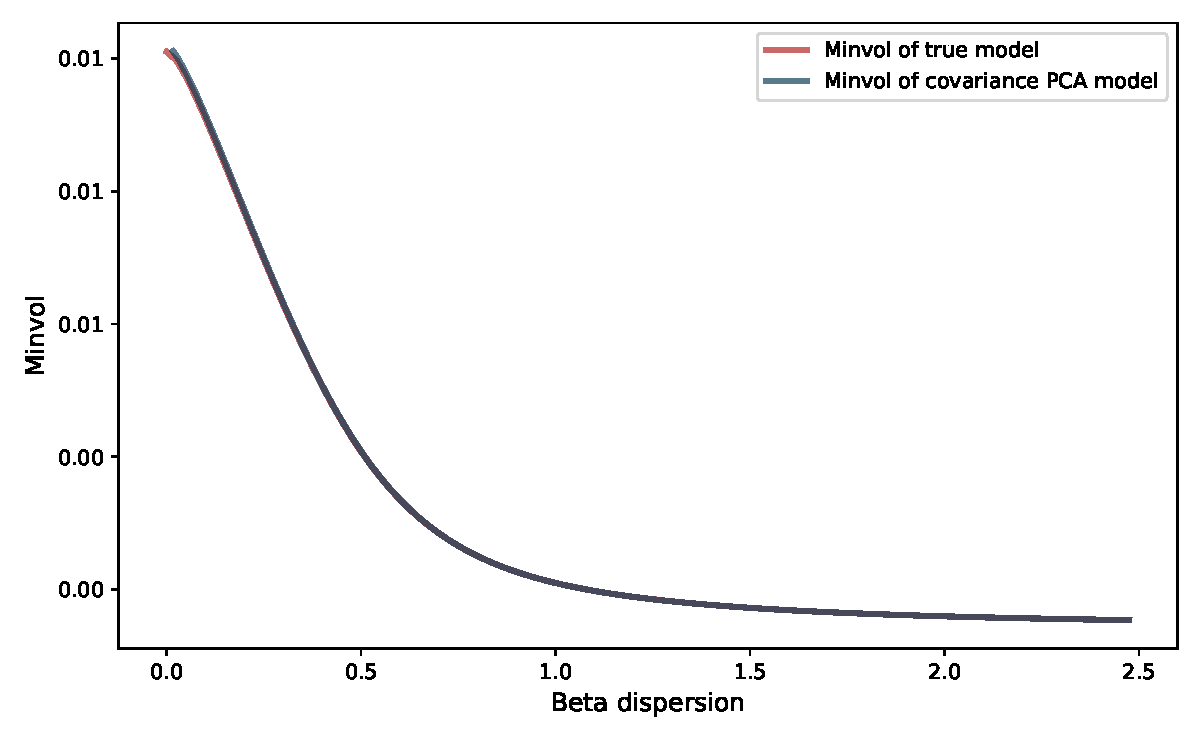
\includegraphics[scale=0.33]{img/DispersionvsPortfolioLOMinvol1factorsN512T256fvol16minsvol30maxsvol90}
  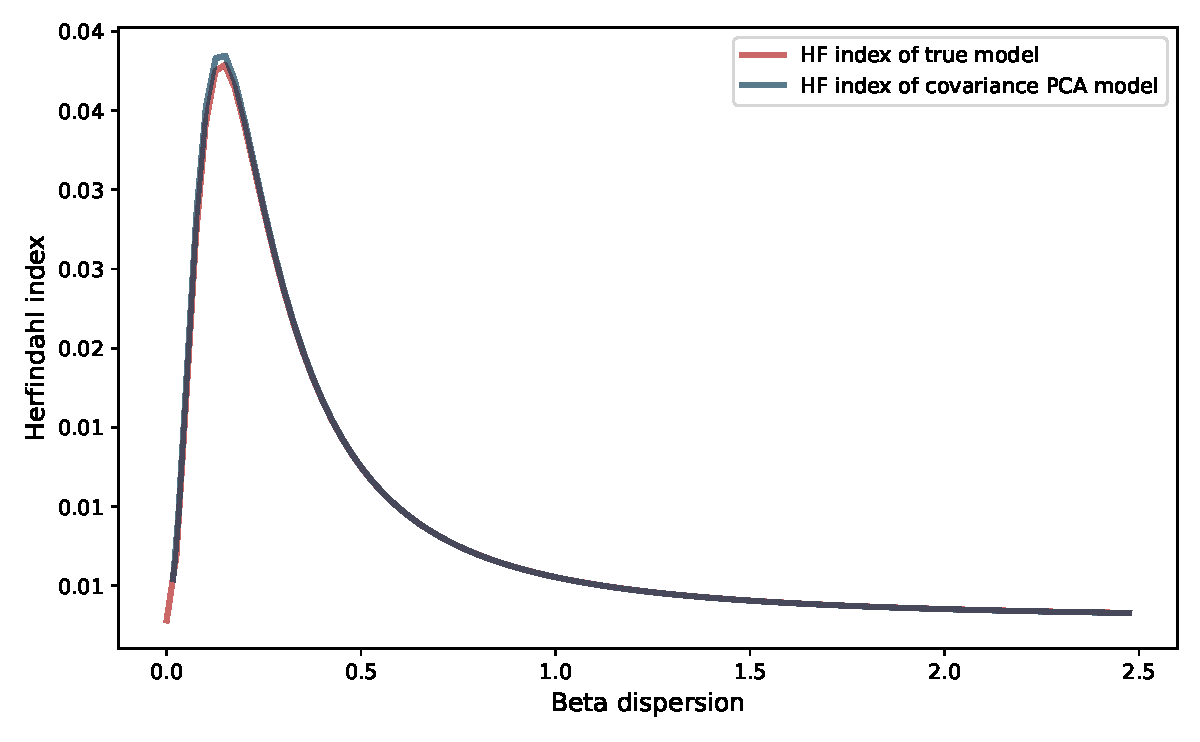
\includegraphics[scale=0.33]{img/DispersionvsLSMinvolHFindex1factorsN512T256fvol16minsvol30maxsvol90}
  \includegraphics[scale=0.33]{img/DispersionvsLOMinvolHFindex1factorsN512T256fvol16minsvol30maxsvol90}
\end{center}
\caption{Beta dispersion
($p = 512$) vs a.p. correlation, skewness, melt up, entropy,
minimum volatility (long short and long only),
and mininum volatility portfolio Herfindahl index
(long short and long only).} 
\end{figure}





\begin{figure}[htp]
\begin{center}
  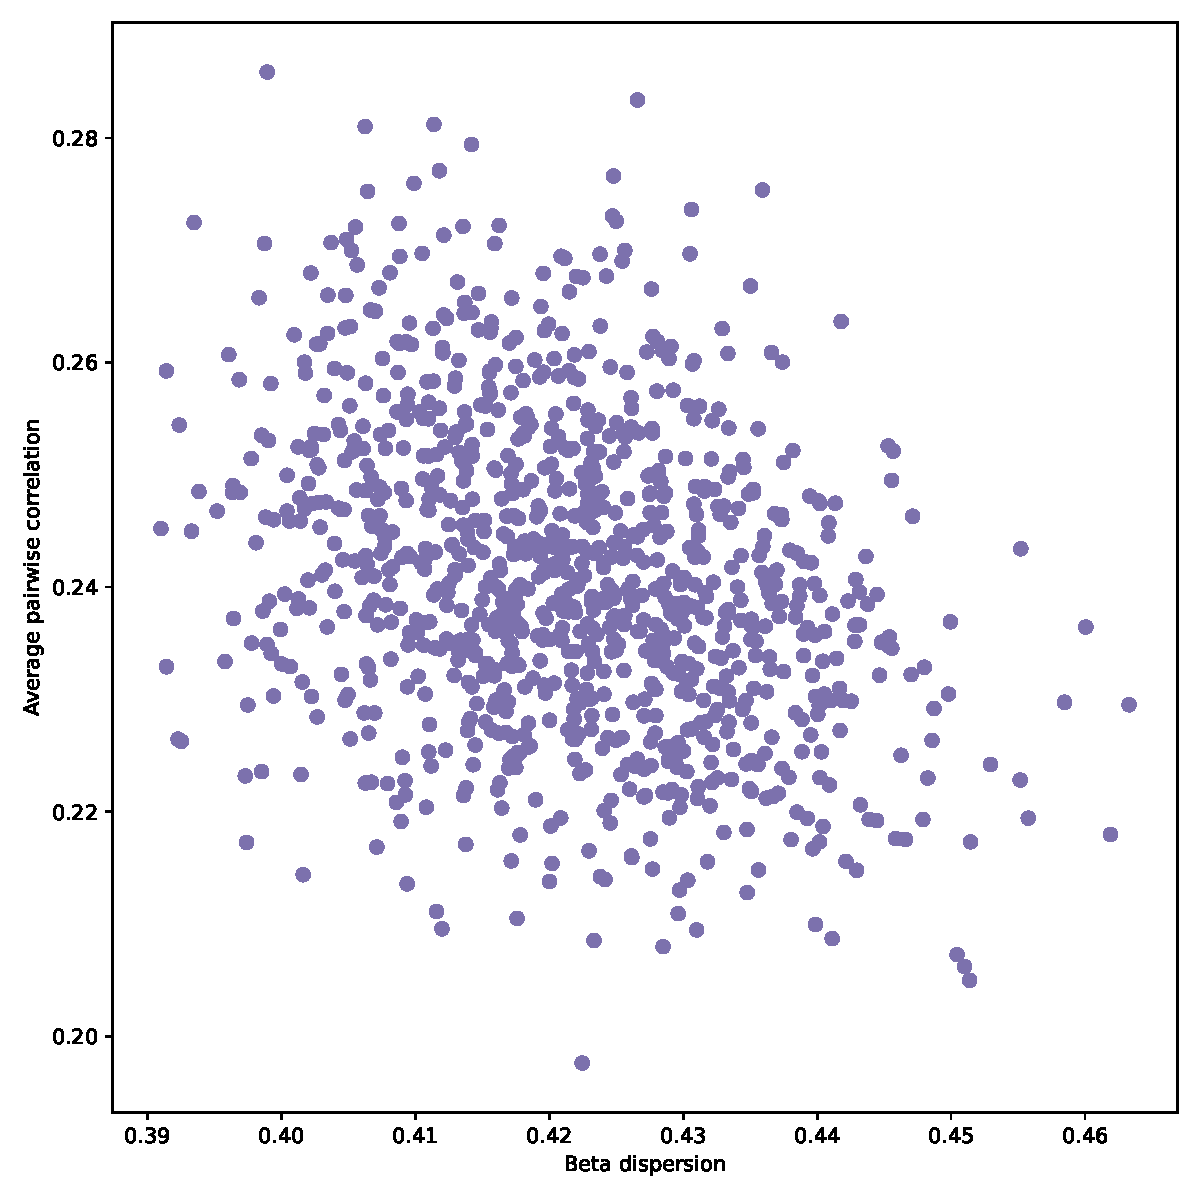
\includegraphics[scale=0.33]{img/SampleCovDispersionvsCorrelation1factorsN128T256disp04fvol16minsvol10maxsvol50}
	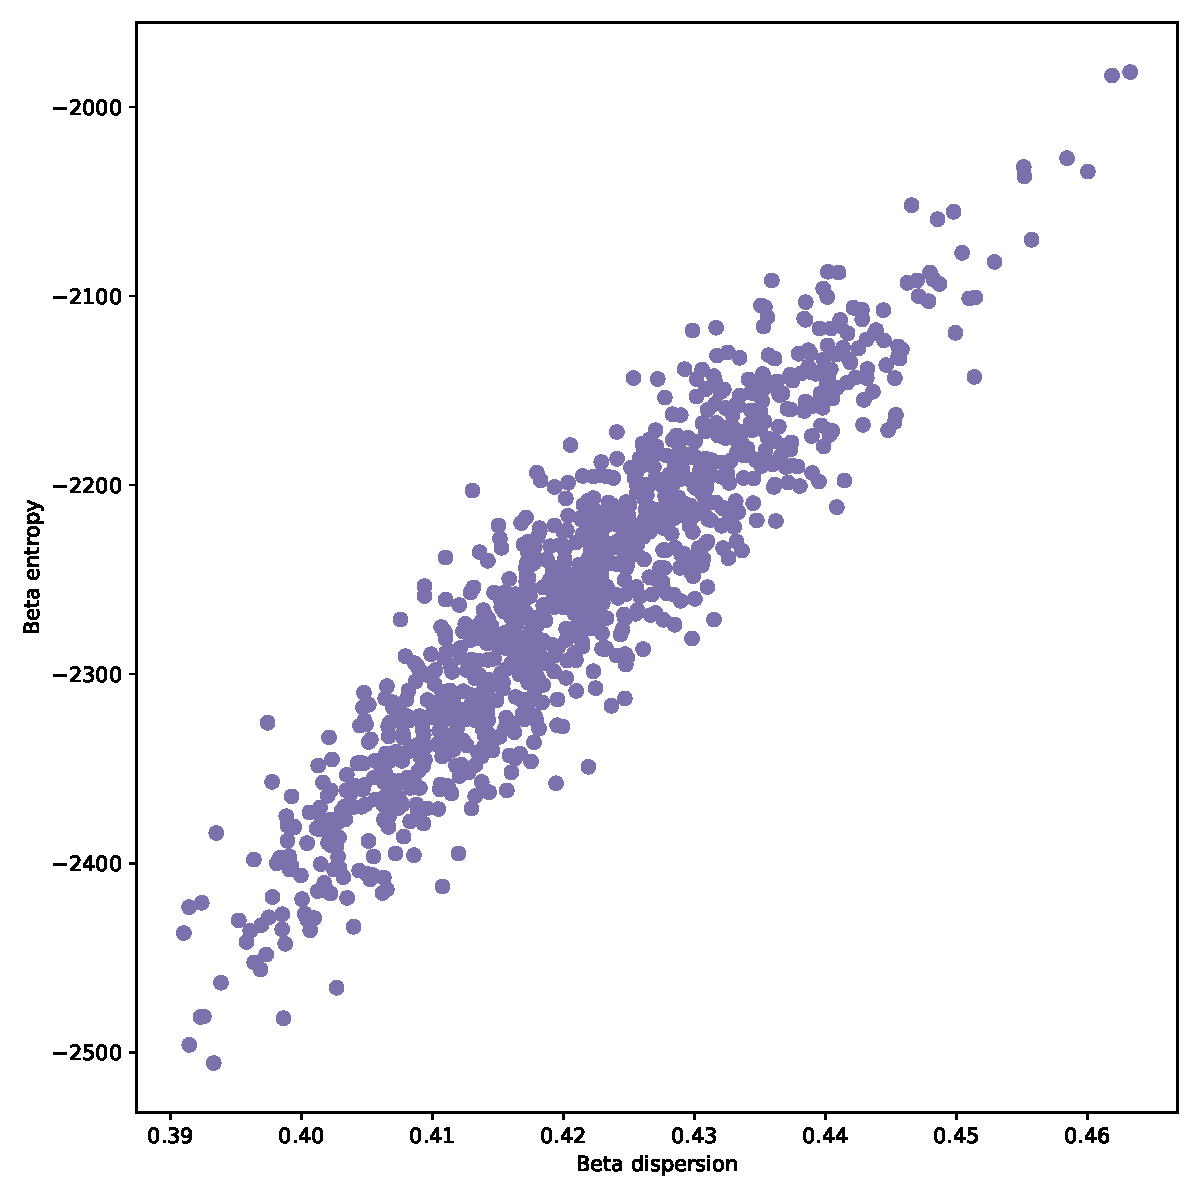
\includegraphics[scale=0.33]{img/SampleCovDispersionvsEntropy1factorsN128T256disp04fvol16minsvol10maxsvol50}
  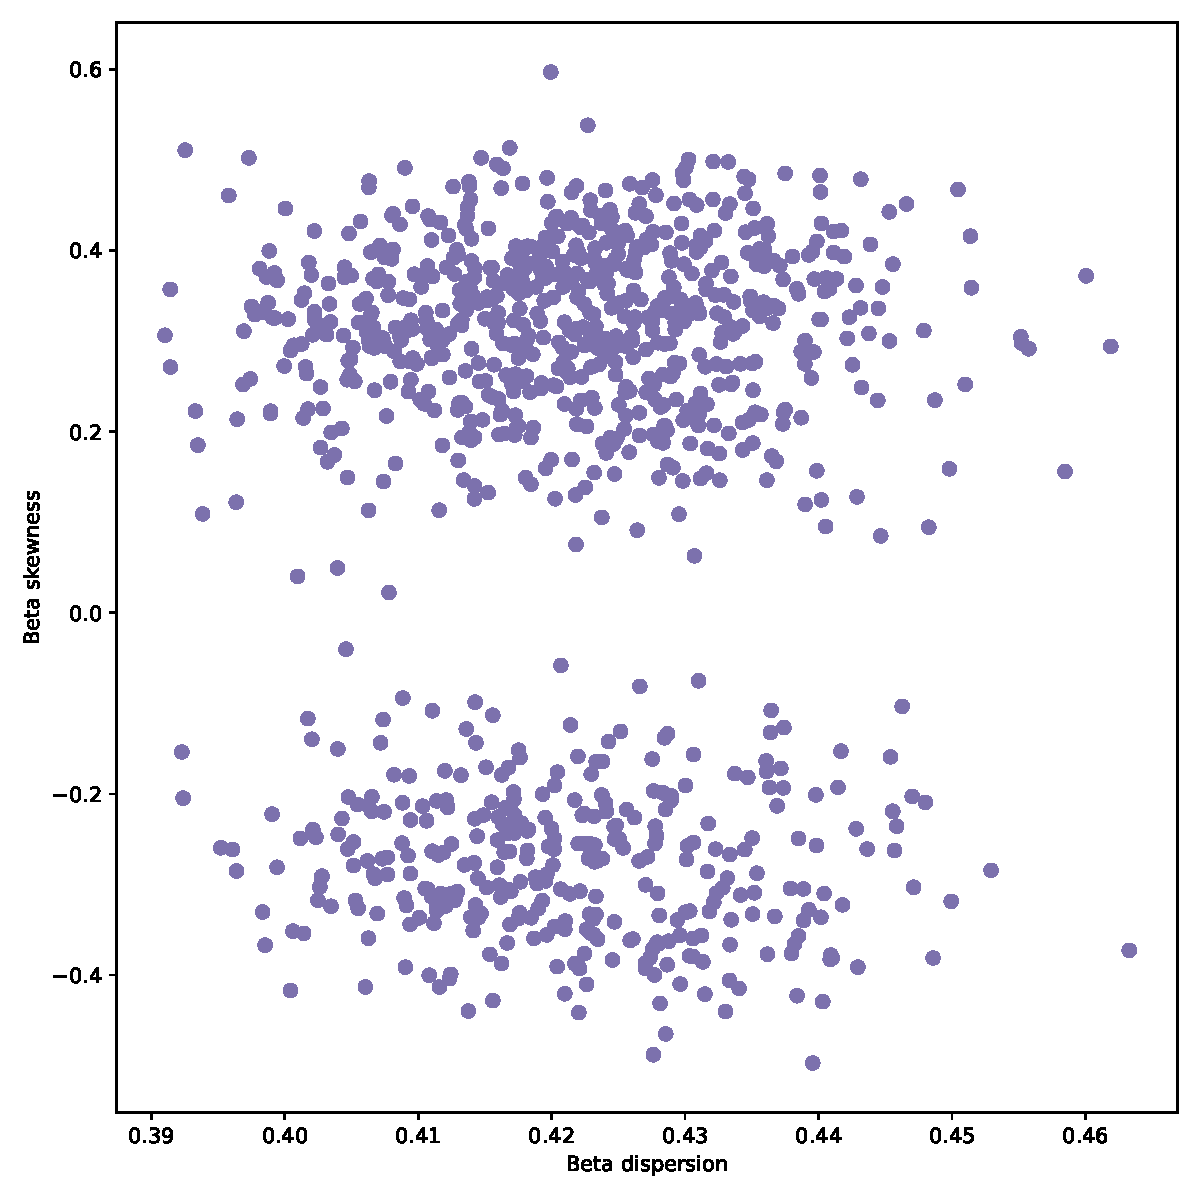
\includegraphics[scale=0.33]{img/SampleCovDispersionvsSkew1factorsN128T256disp04fvol16minsvol10maxsvol50}
  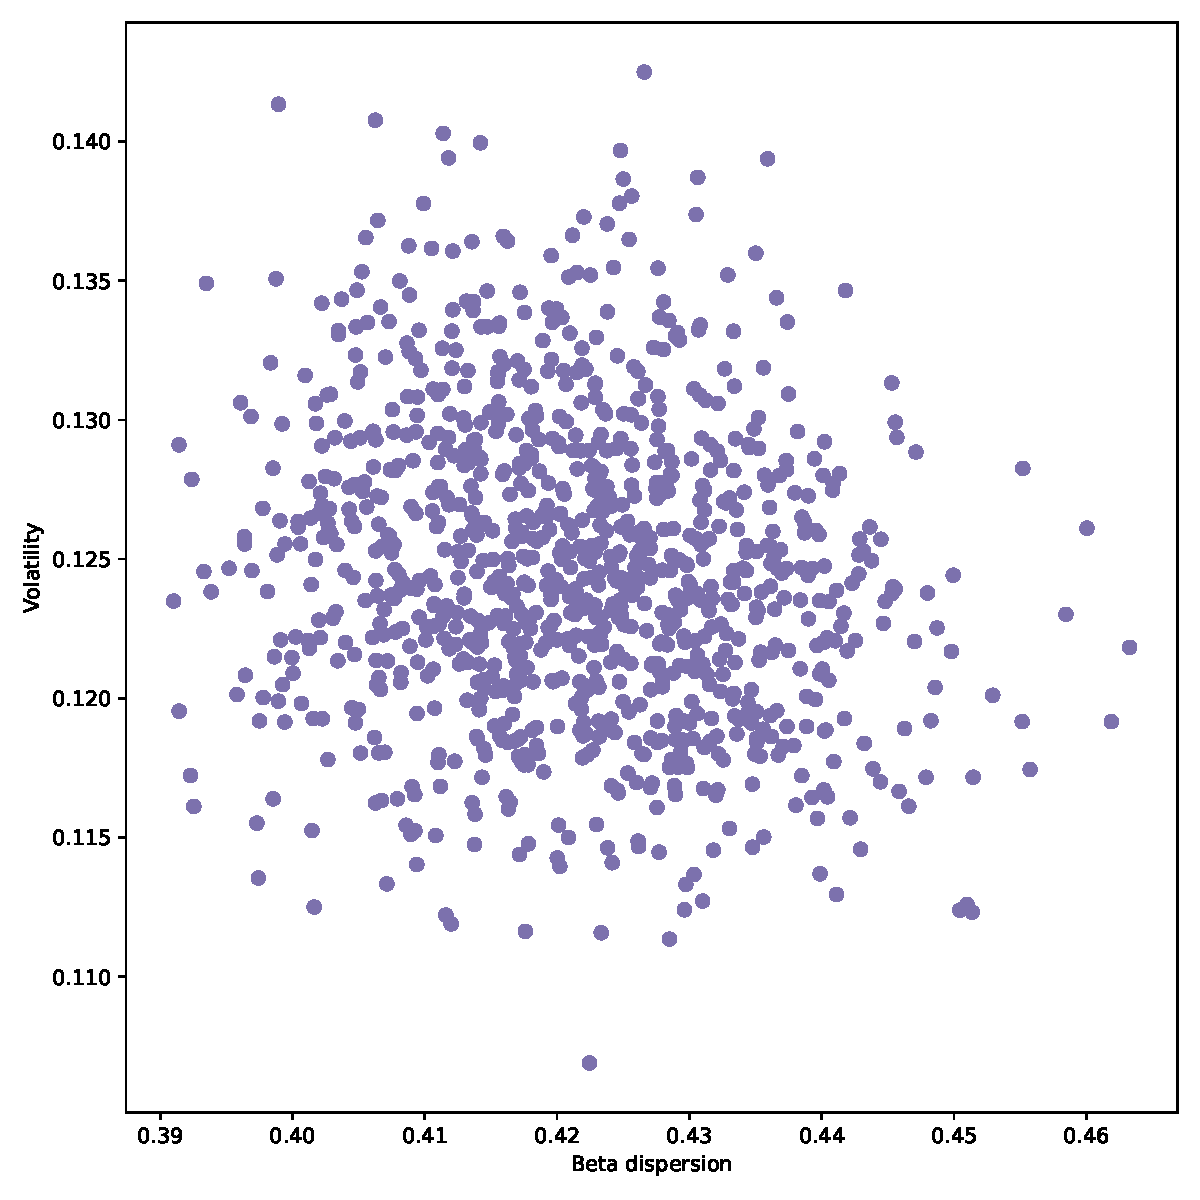
\includegraphics[scale=0.33]{img/SampleCovDispersionvsVolatility1factorsN128T256disp04fvol16minsvol10maxsvol50}
\end{center}
\caption{Sample scatter plots for covariance PCA.
($p = 512, n = 128$). Model 
$(\rmd^2(\beta), \sigma_\rmM, \text{ave}(\delta))
= (0.4, 16, 0.4)$.} 
\end{figure}





\begin{figure}[htp]
\begin{center}
  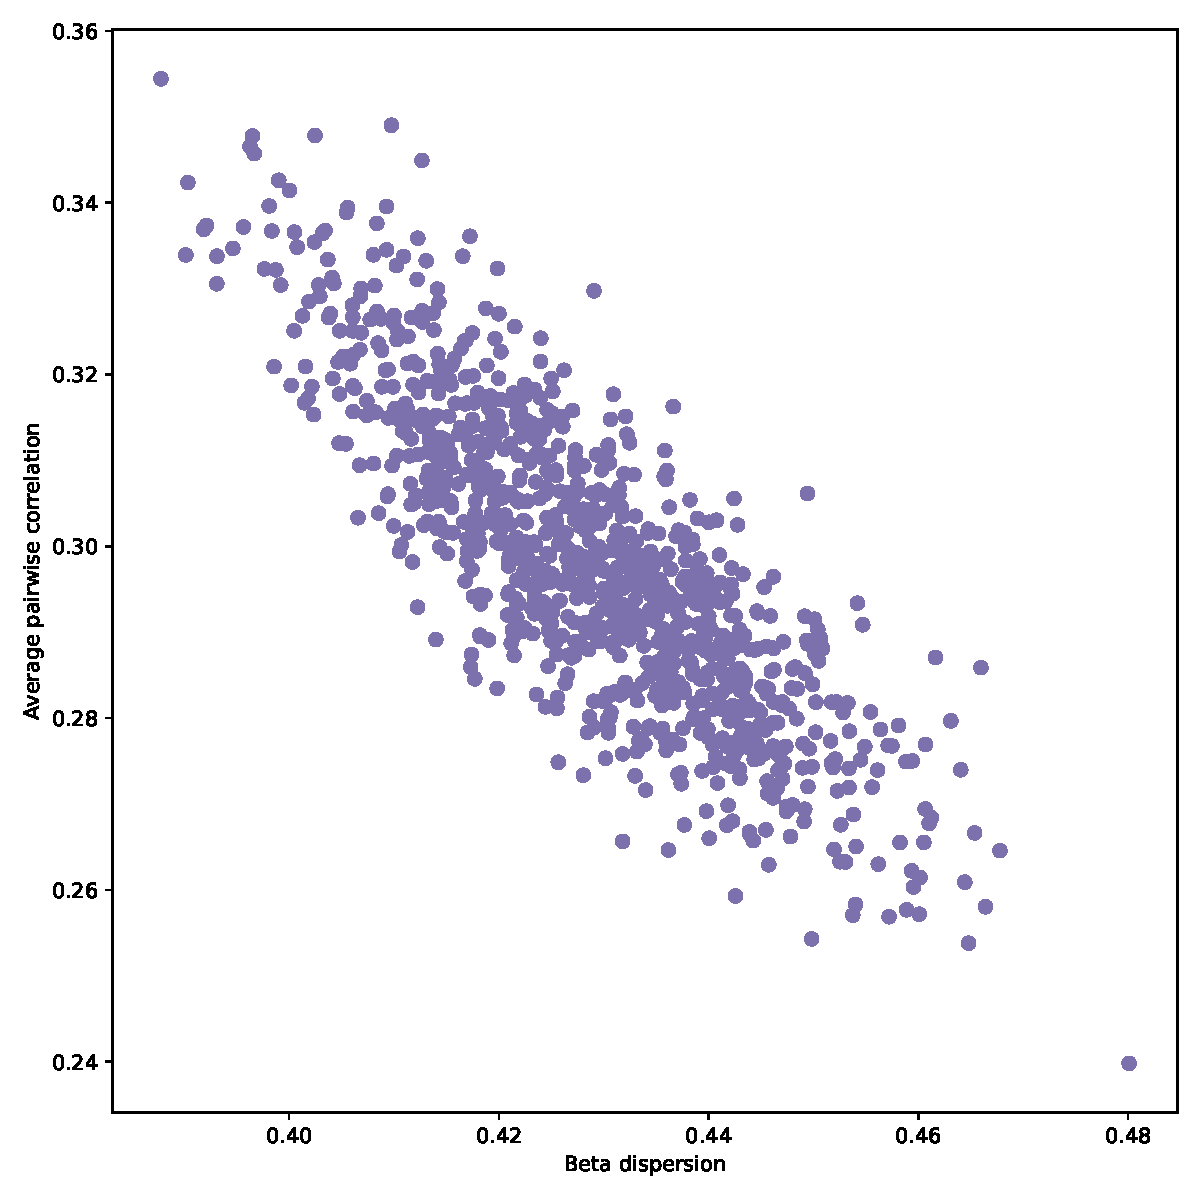
\includegraphics[scale=0.33]{img/SampleCorDispersionvsCorrelation1factorsN128T256disp04fvol16minsvol10maxsvol50}
	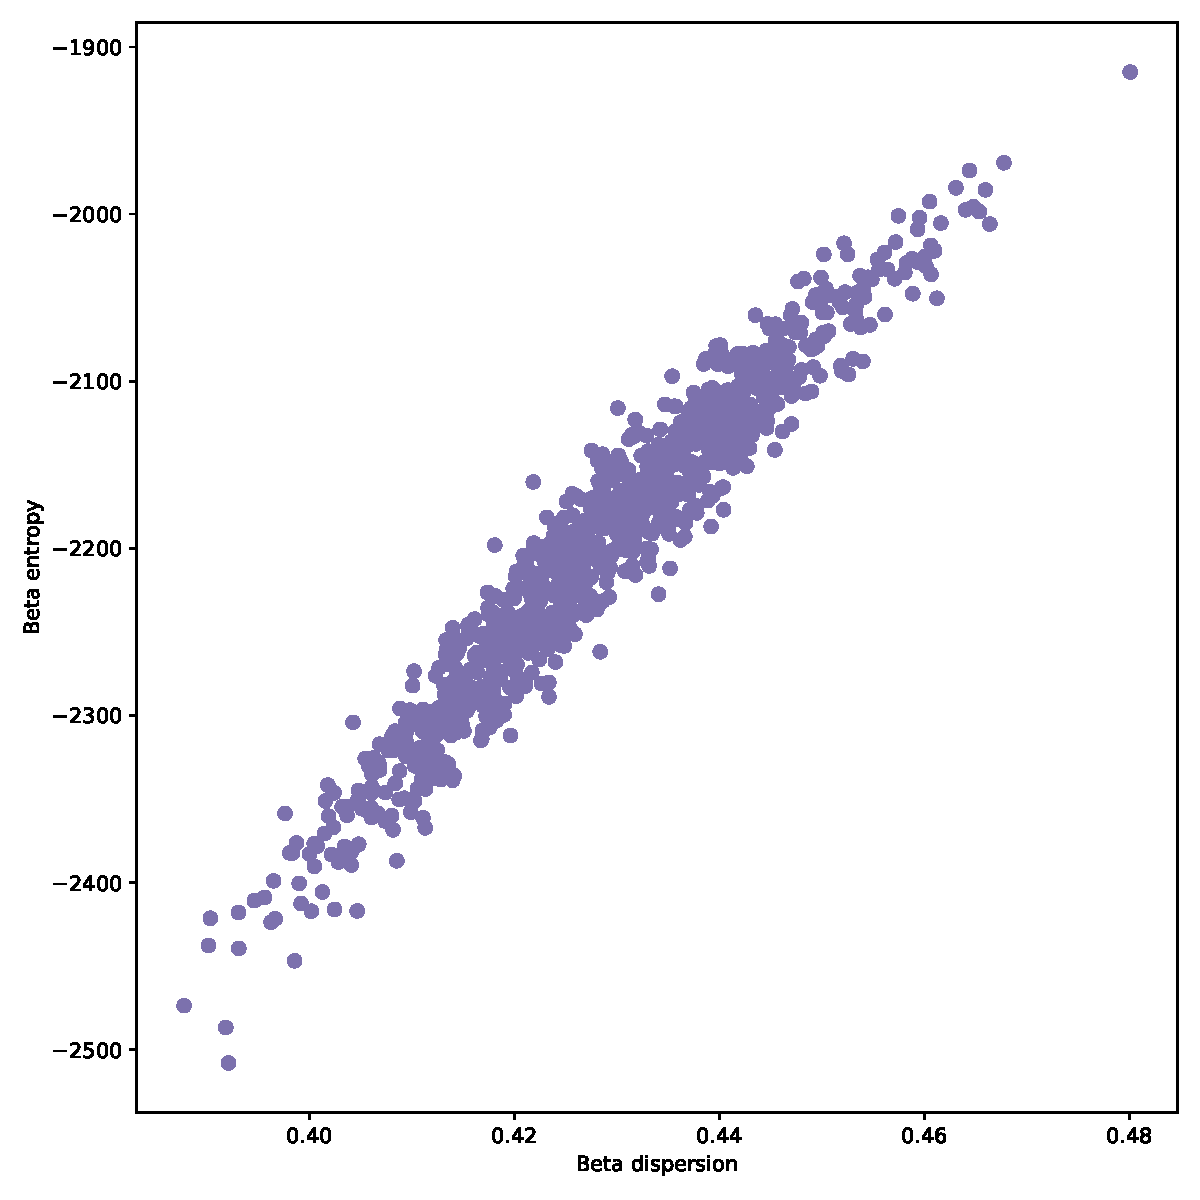
\includegraphics[scale=0.33]{img/SampleCorDispersionvsEntropy1factorsN128T256disp04fvol16minsvol10maxsvol50}
  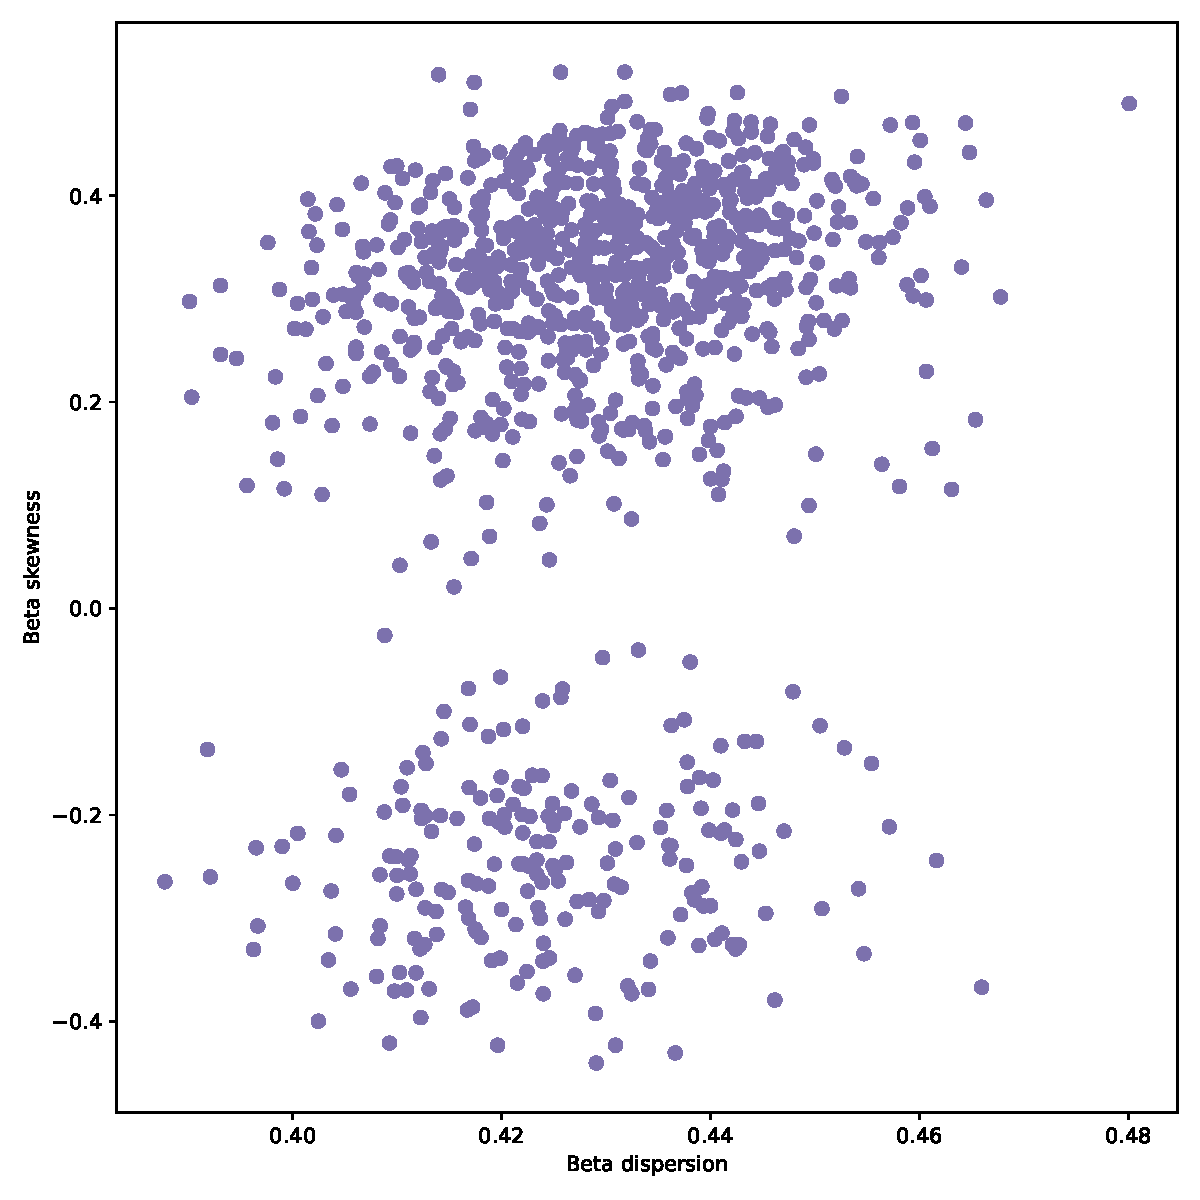
\includegraphics[scale=0.33]{img/SampleCorDispersionvsSkew1factorsN128T256disp04fvol16minsvol10maxsvol50}
  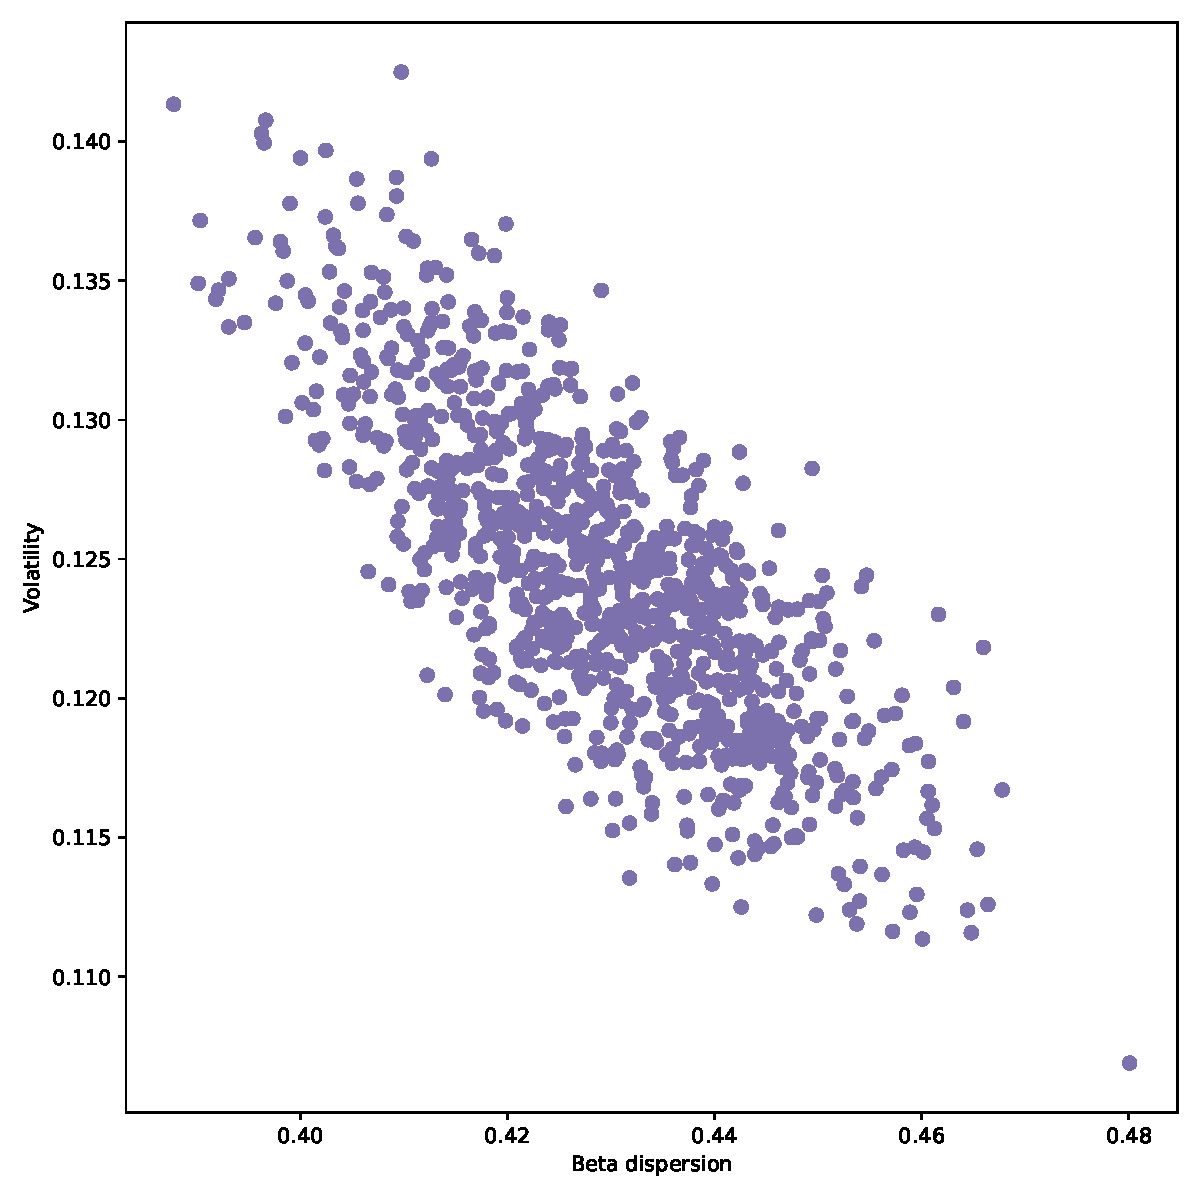
\includegraphics[scale=0.33]{img/SampleCorDispersionvsVolatility1factorsN128T256disp04fvol16minsvol10maxsvol50}
\end{center}
\caption{Sample scatter plots for correlation PCA.
($p = 512, n = 128$). Model 
$(\rmd^2(\beta), \sigma_\rmM, \text{ave}(\delta))
= (0.4, 16, 0.4)$.} 
\end{figure}


\newpage


\section{Empirics}


\begin{enumerate}
  \item High beta dispersion is a sign of financial stress.
  \item Mean beta is mean-reverting (business cycles).
  \item In crisis all correlations {\bf do not} go to one
  (anti-Markowitz).
  \item Melt-up and beta dispersion are associated with
   market bubbles.
  \item Skewness, entropy, etc.
\end{enumerate}


\begin{figure}[htp]
\begin{center}
  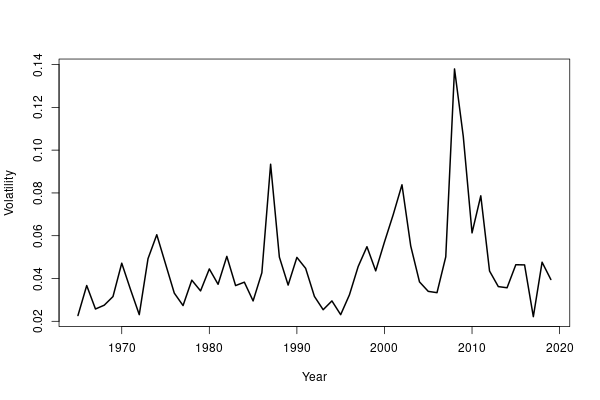
\includegraphics[scale=0.33]{img/plot1}
  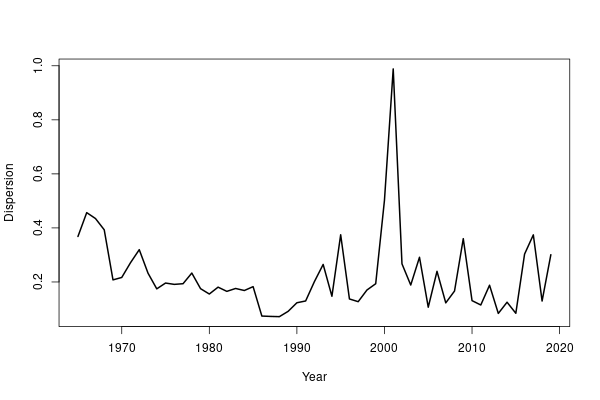
\includegraphics[scale=0.33]{img/plot2}
  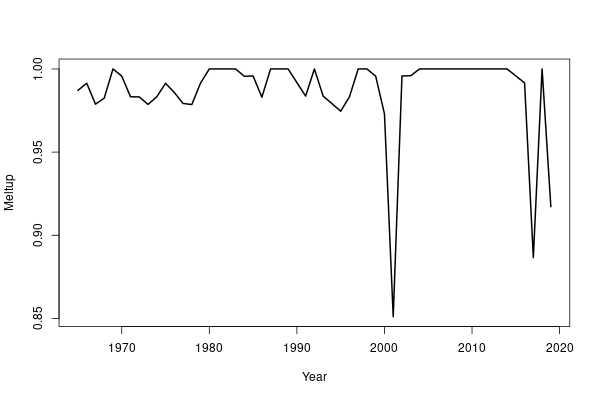
\includegraphics[scale=0.33]{img/plot3}
  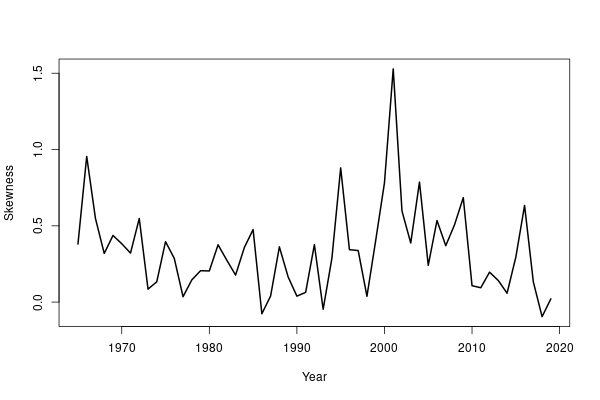
\includegraphics[scale=0.33]{img/plot4}
  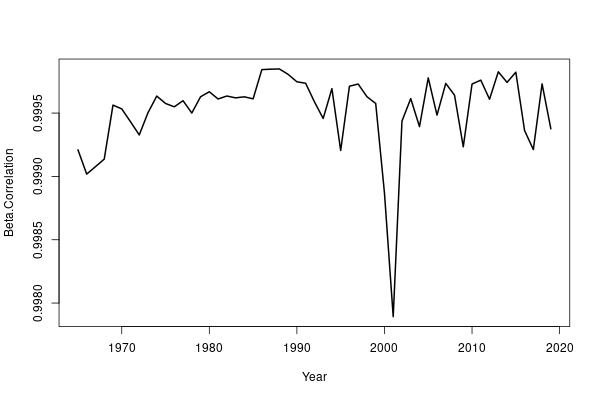
\includegraphics[scale=0.33]{img/plot5}
  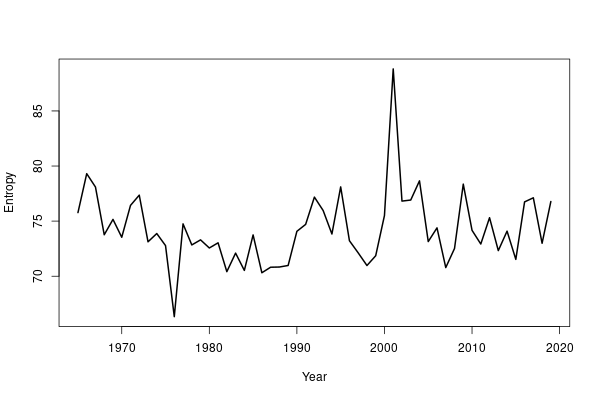
\includegraphics[scale=0.33]{img/plot6}
\end{center}
\caption{S\&P 500 data from 1965-2019.}
\end{figure}


\section{Regime models}

\section{Multi-index and graphical models}

\section{Asset return distributions}

\newpage

\appendix

\section{Beta dispersion vs Skew, Melt up, Correlation, Entropy
plots}

\begin{figure}[htp]
\begin{center}
  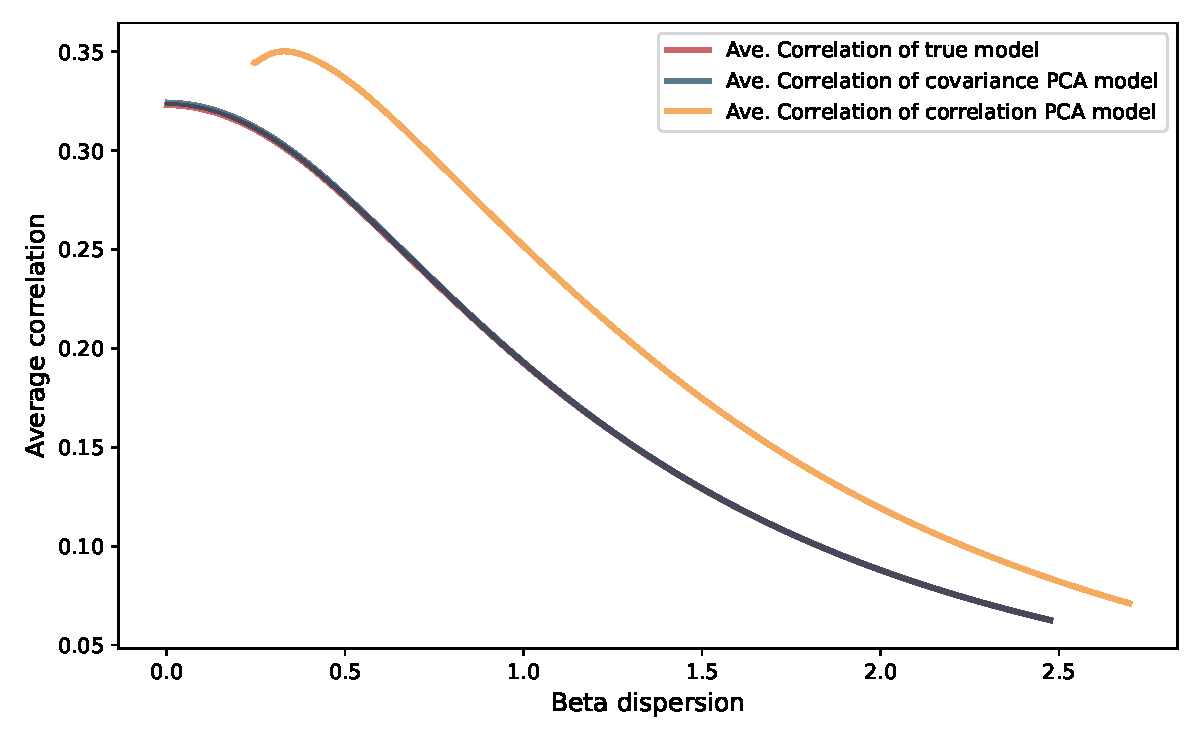
\includegraphics[scale=0.33]{img/DispersionvsCorrelation1factorsN512T256fvol16minsvol10maxsvol40}
  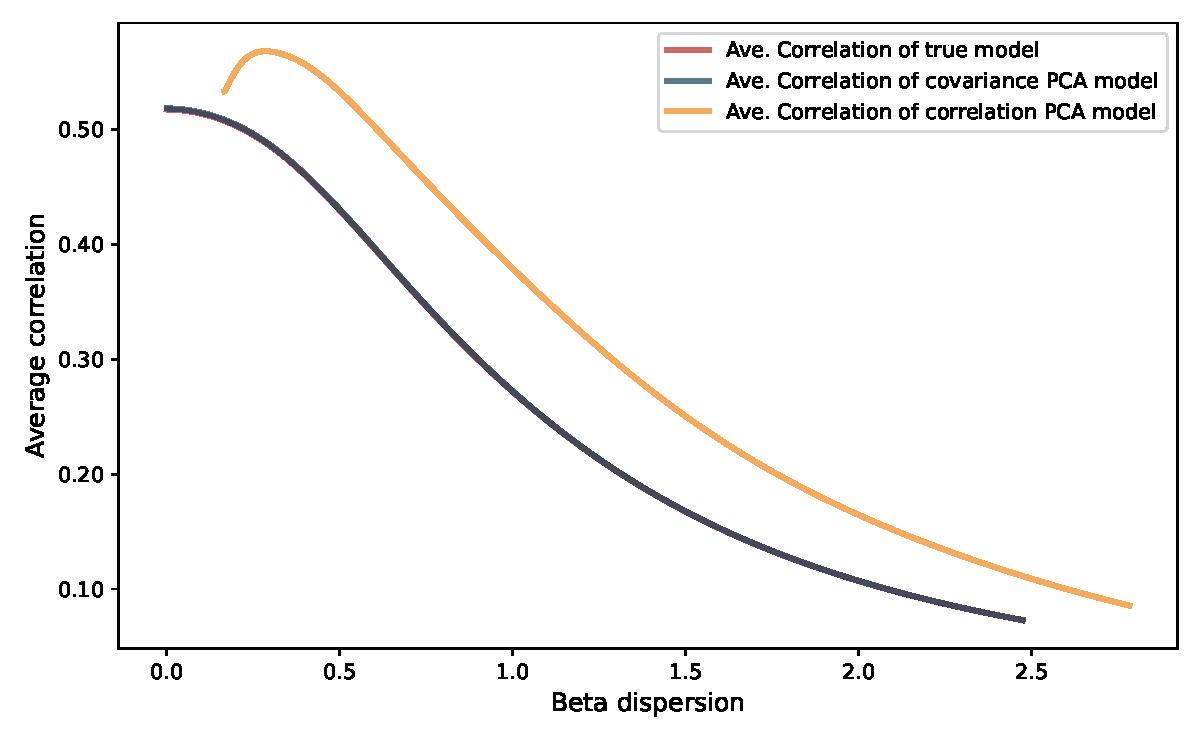
\includegraphics[scale=0.33]{img/DispersionvsCorrelation1factorsN512T256fvol25minsvol10maxsvol40}
  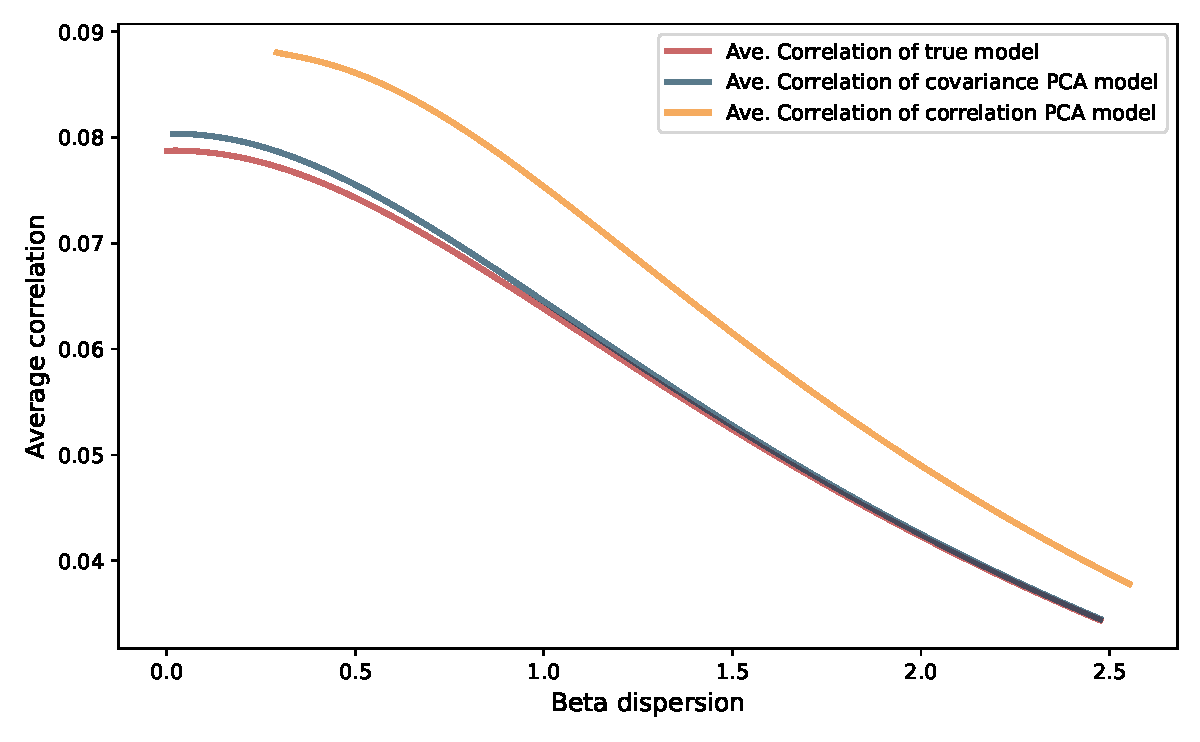
\includegraphics[scale=0.33]{img/DispersionvsCorrelation1factorsN512T256fvol16minsvol30maxsvol90}
  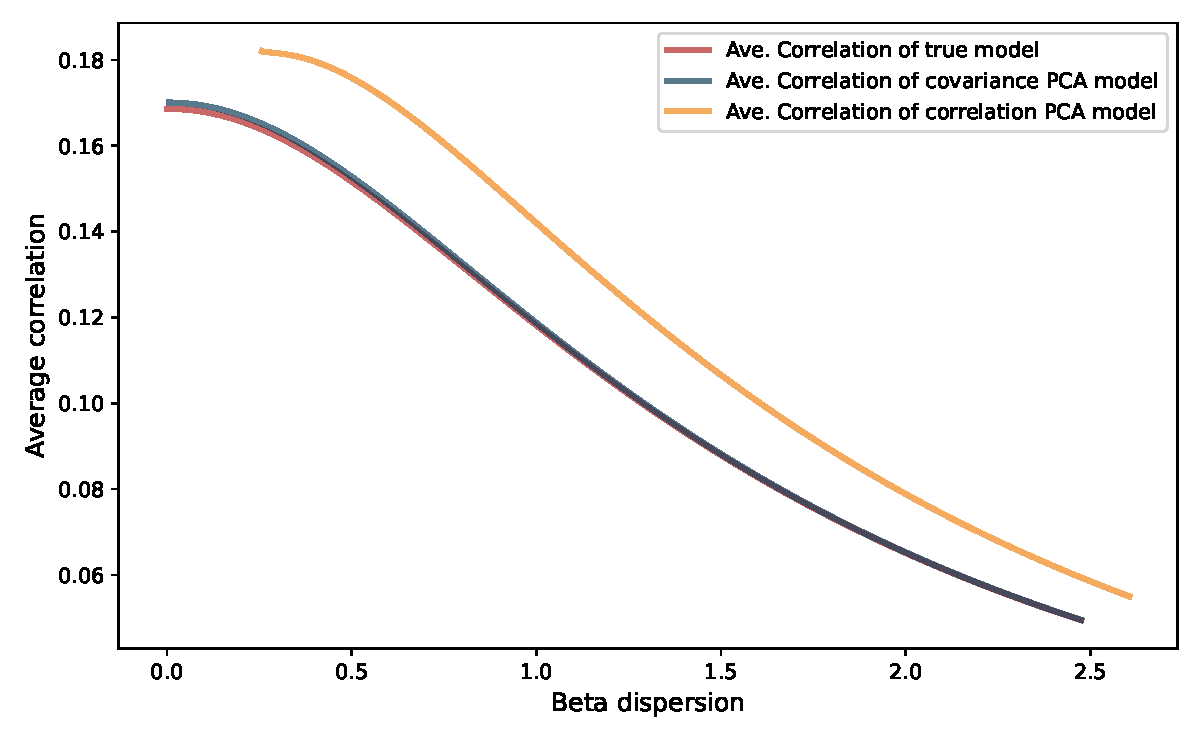
\includegraphics[scale=0.33]{img/DispersionvsCorrelation1factorsN512T256fvol25minsvol30maxsvol90}
\end{center}
\caption{Average pairwise correlation vs Beta dispersion
($p = 512$). 
Top left: $(\sigma_\rmM, \text{ave}(\delta)) = (16,25)$.
Top right: $(\sigma_\rmM, \text{ave}(\delta)) = (25,25)$.
Bottom left: $(\sigma_\rmM, \text{ave}(\delta)) = (16,60)$.
Bottom left: $(\sigma_\rmM, \text{ave}(\delta)) = (25,60)$.
Volatility units are percent annualized.}
\end{figure}


\begin{figure}[htp]
\begin{center}
  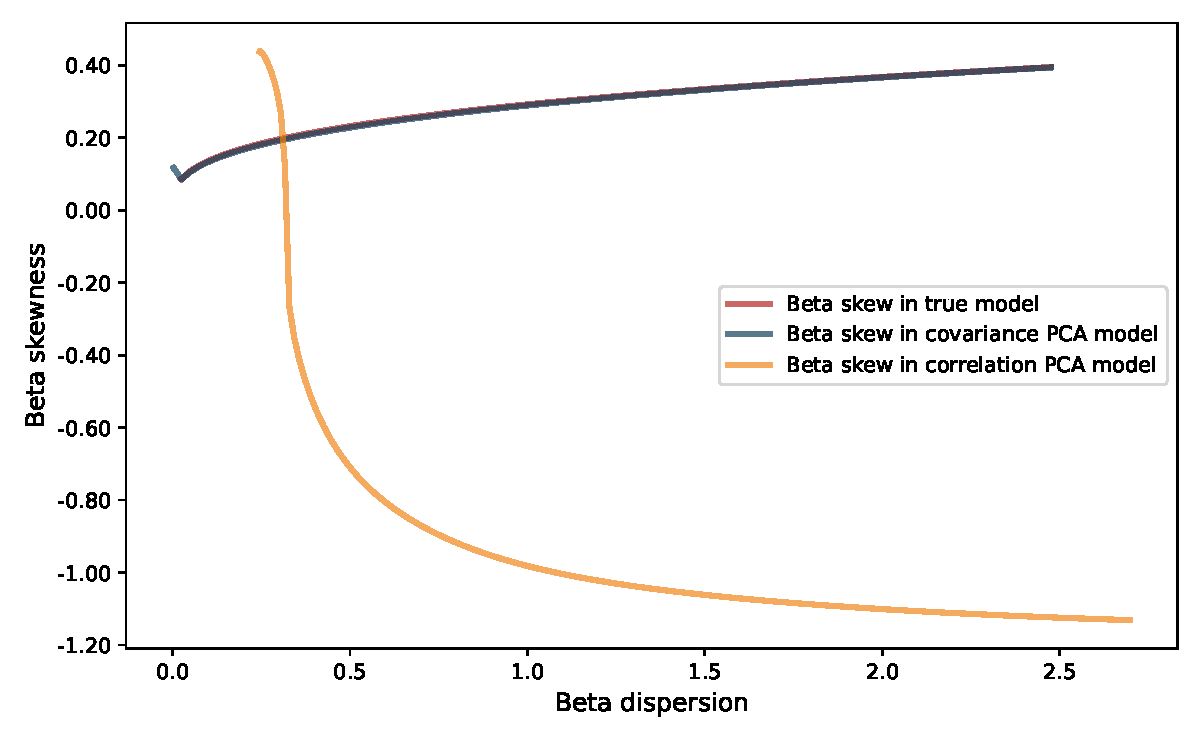
\includegraphics[scale=0.33]{img/DispersionvsSkew1factorsN512T256fvol16minsvol10maxsvol40}
  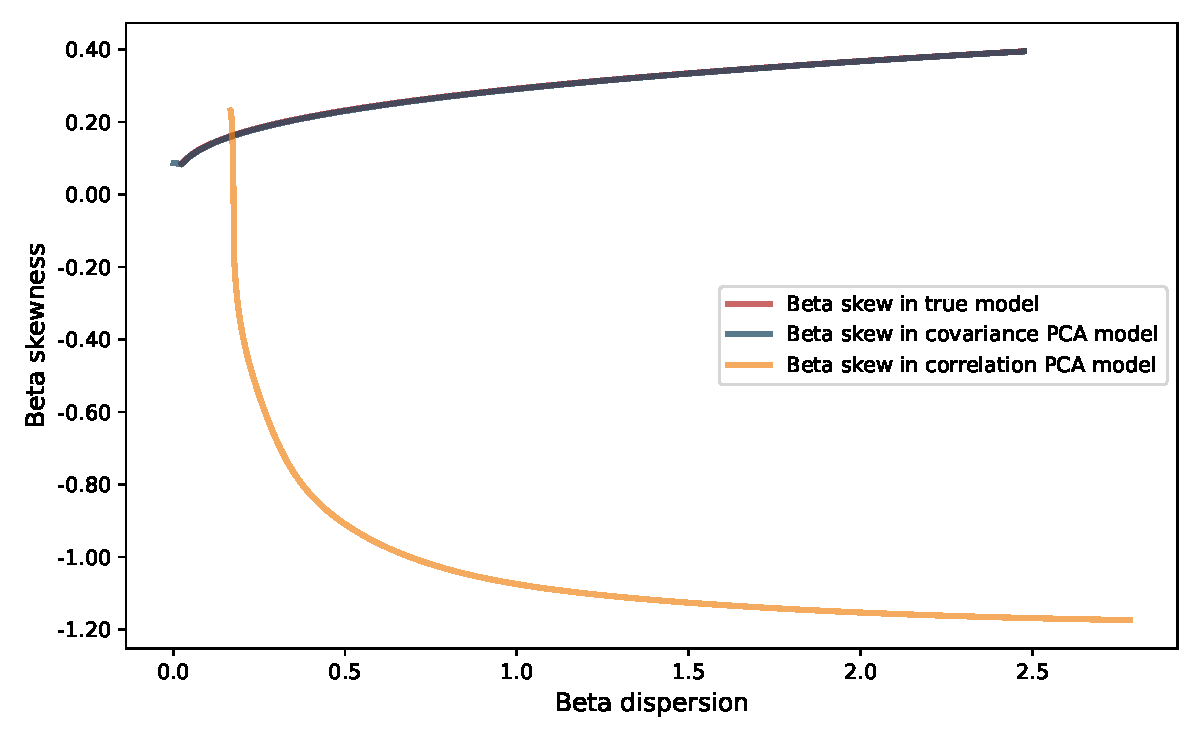
\includegraphics[scale=0.33]{img/DispersionvsSkew1factorsN512T256fvol25minsvol10maxsvol40}
  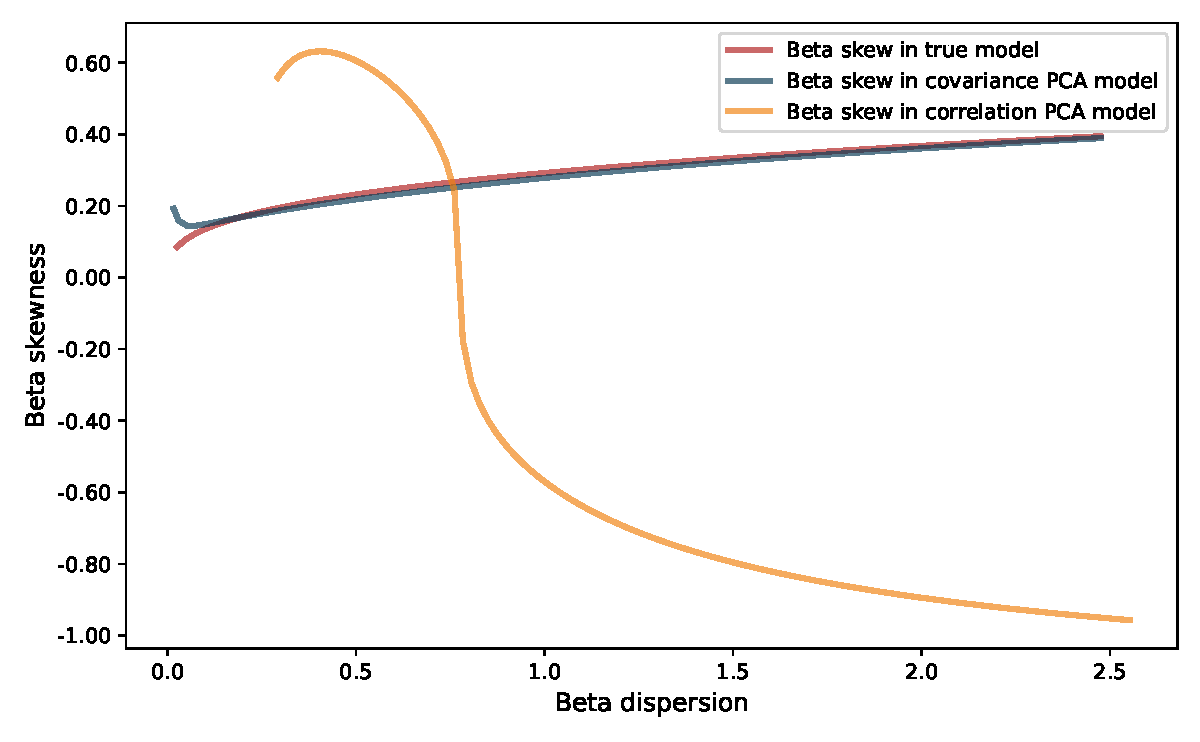
\includegraphics[scale=0.33]{img/DispersionvsSkew1factorsN512T256fvol16minsvol30maxsvol90}
  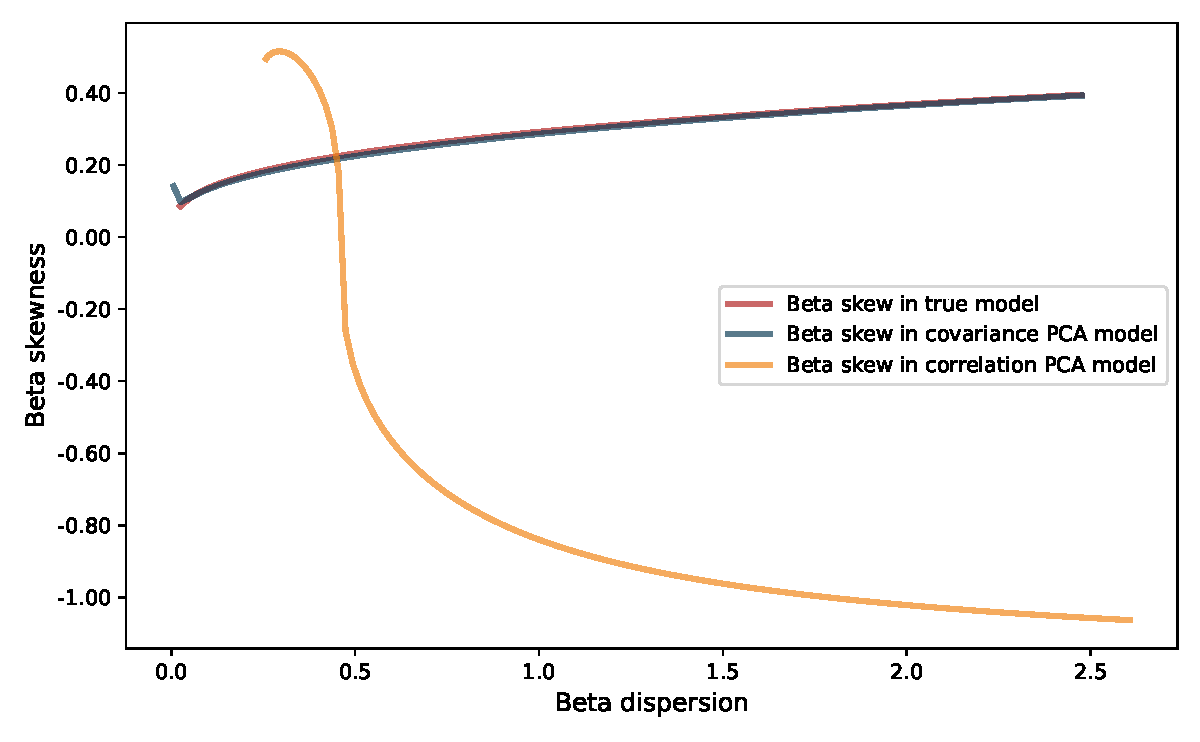
\includegraphics[scale=0.33]{img/DispersionvsSkew1factorsN512T256fvol25minsvol30maxsvol90}
\end{center}
\caption{Beta Skewness vs Beta dispersion
($p = 512$). 
Top left: $(\sigma_\rmM, \text{ave}(\delta)) = (16,25)$.
Top right: $(\sigma_\rmM, \text{ave}(\delta)) = (25,25)$.
Bottom left: $(\sigma_\rmM, \text{ave}(\delta)) = (16,60)$.
Bottom left: $(\sigma_\rmM, \text{ave}(\delta)) = (25,60)$.
Volatility units are percent annualized.}
\end{figure}


\begin{figure}[htp]
\begin{center}
  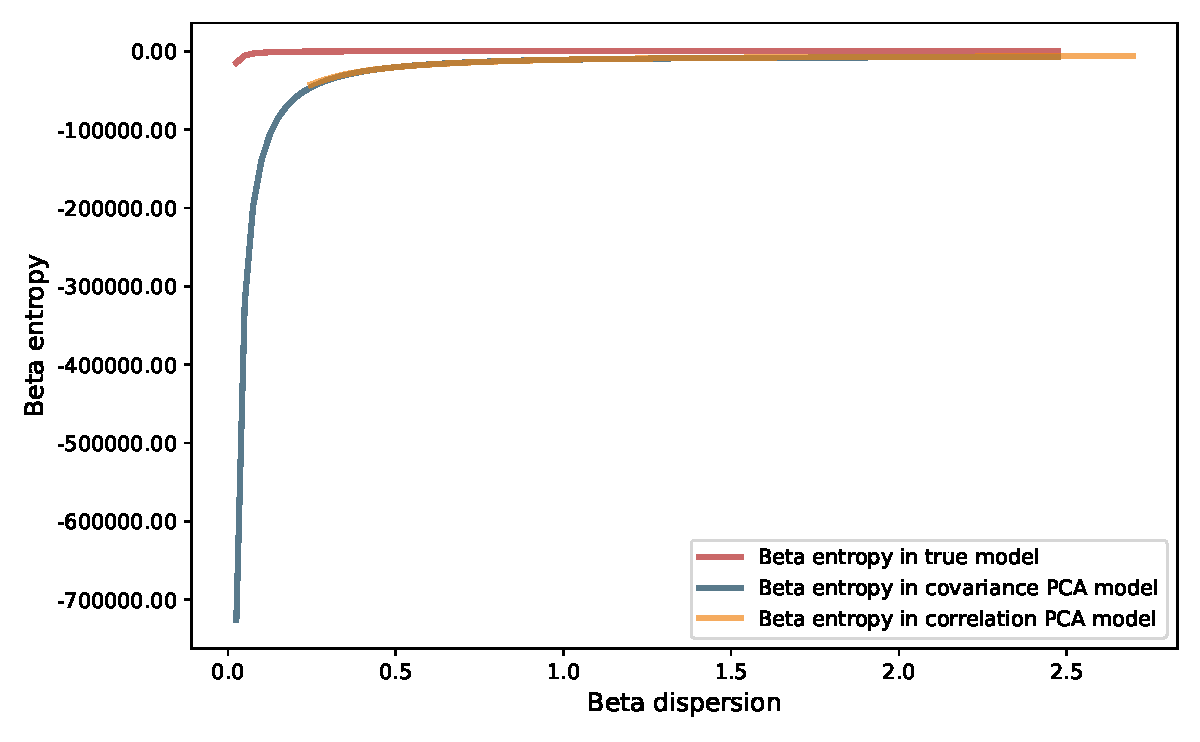
\includegraphics[scale=0.33]{img/DispersionvsEntropy1factorsN512T256fvol16minsvol10maxsvol40}
  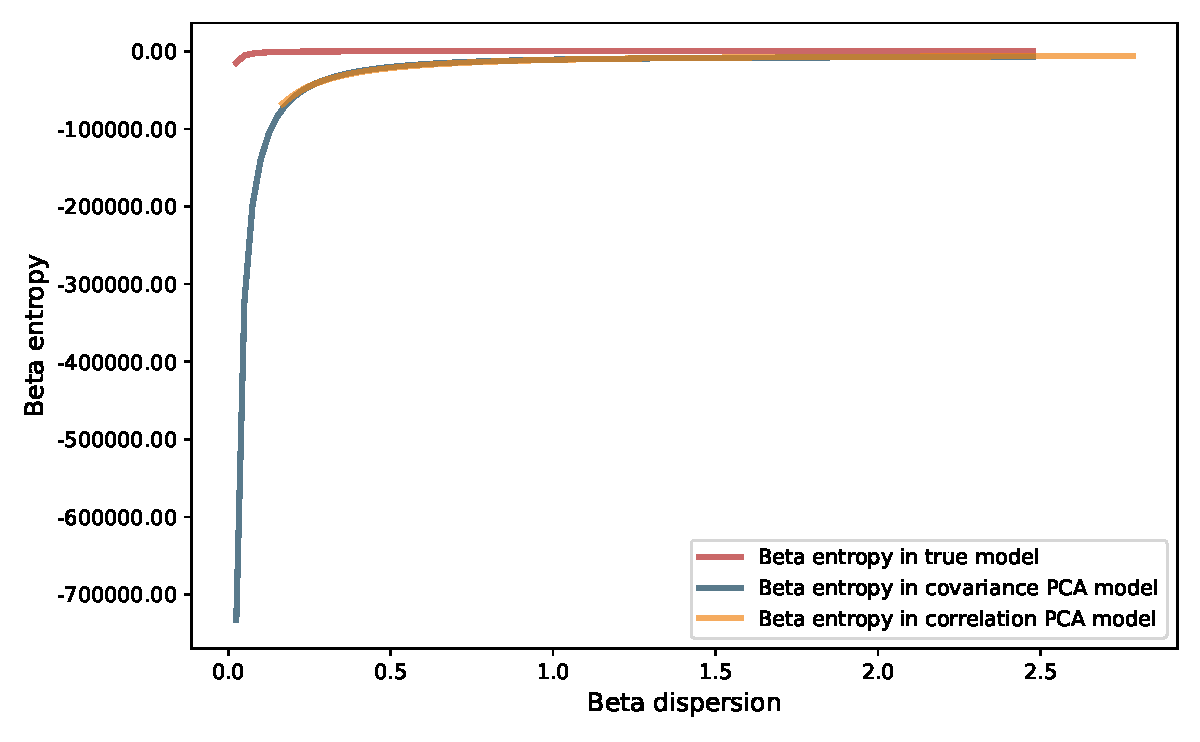
\includegraphics[scale=0.33]{img/DispersionvsEntropy1factorsN512T256fvol25minsvol10maxsvol40}
  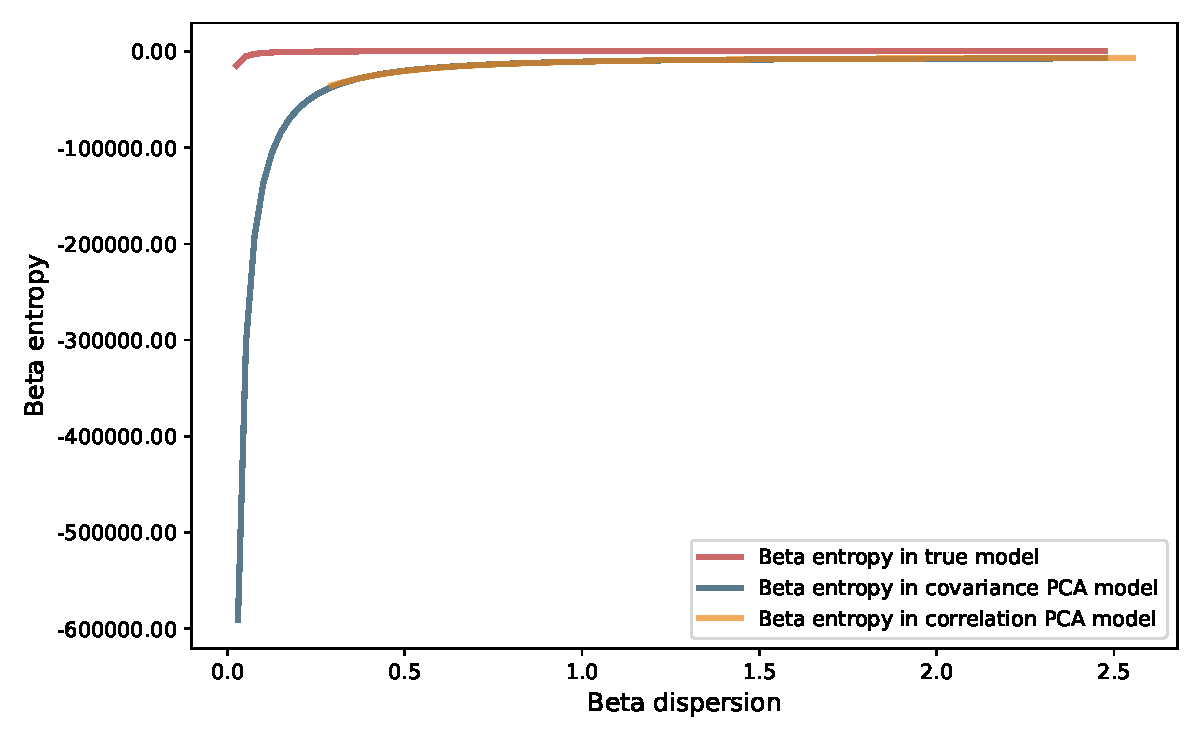
\includegraphics[scale=0.33]{img/DispersionvsEntropy1factorsN512T256fvol16minsvol30maxsvol90}
  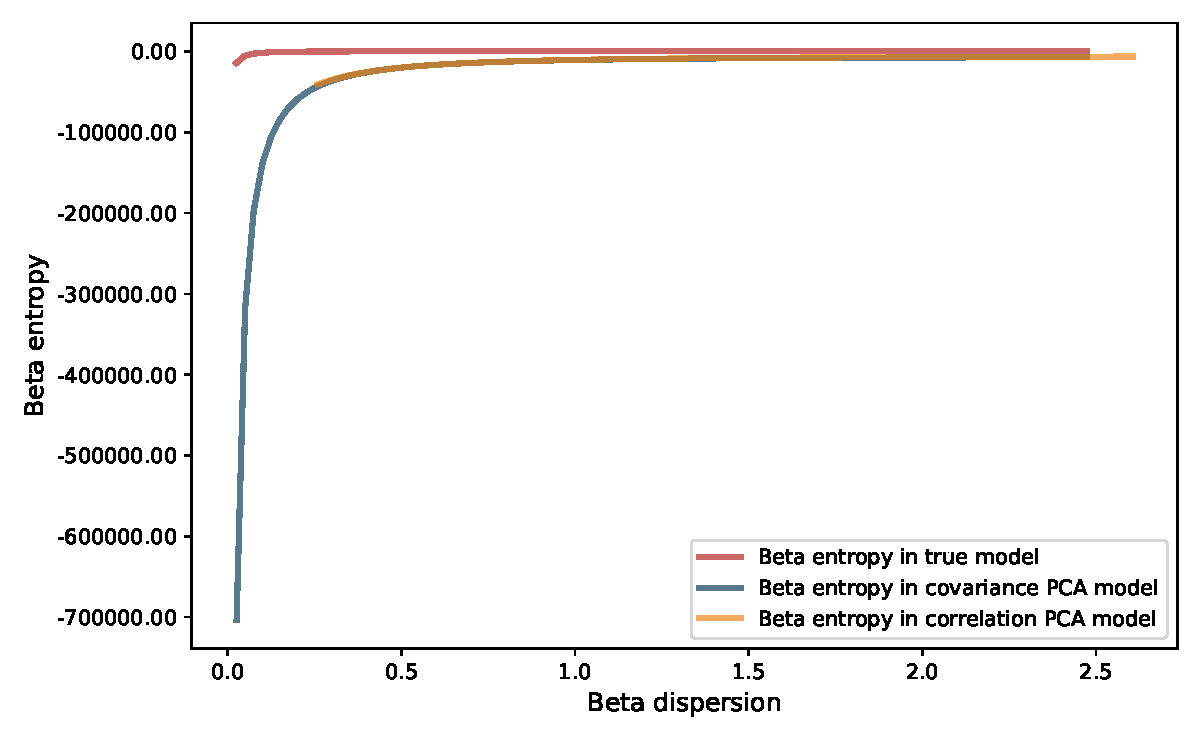
\includegraphics[scale=0.33]{img/DispersionvsEntropy1factorsN512T256fvol25minsvol30maxsvol90}
\end{center}
\caption{Beta Skewness vs Beta dispersion
($p = 512$). 
Top left: $(\sigma_\rmM, \text{ave}(\delta)) = (16,25)$.
Top right: $(\sigma_\rmM, \text{ave}(\delta)) = (25,25)$.
Bottom left: $(\sigma_\rmM, \text{ave}(\delta)) = (16,60)$.
Bottom left: $(\sigma_\rmM, \text{ave}(\delta)) = (25,60)$.
Volatility units are percent annualized.}
\end{figure}

\begin{figure}[htp]
\begin{center}
  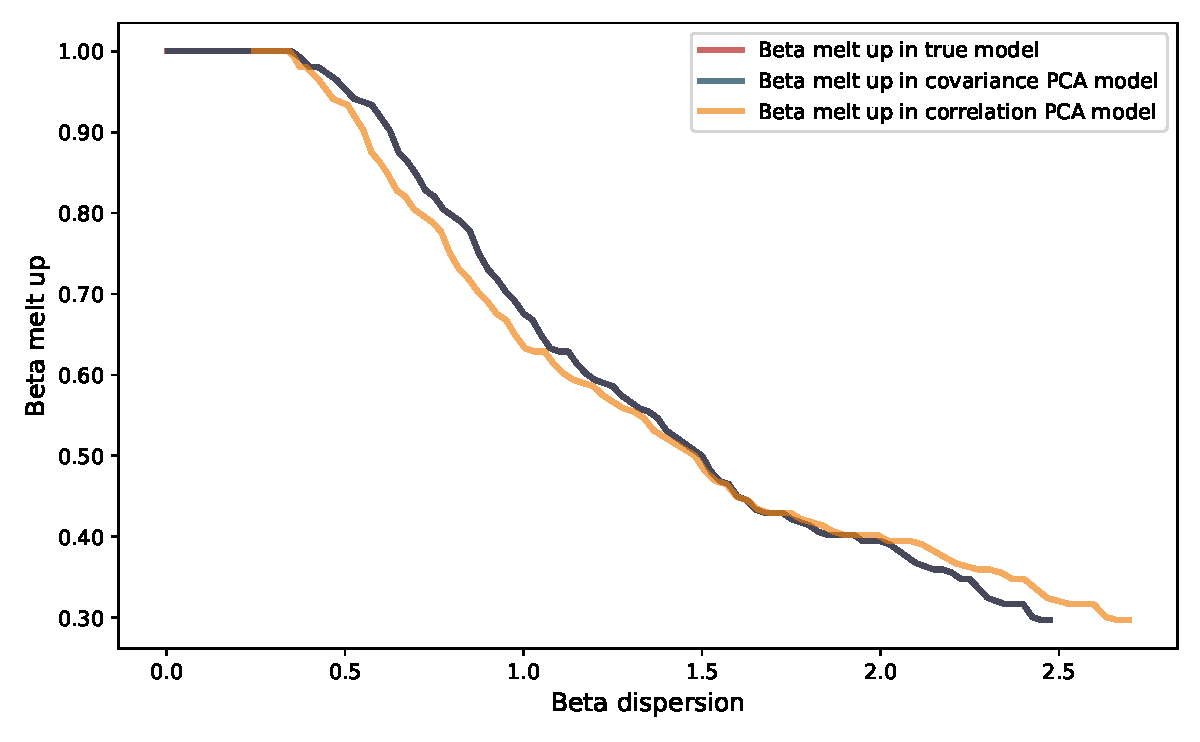
\includegraphics[scale=0.33]{img/DispersionvsMeltup1factorsN512T256fvol16minsvol10maxsvol40}
  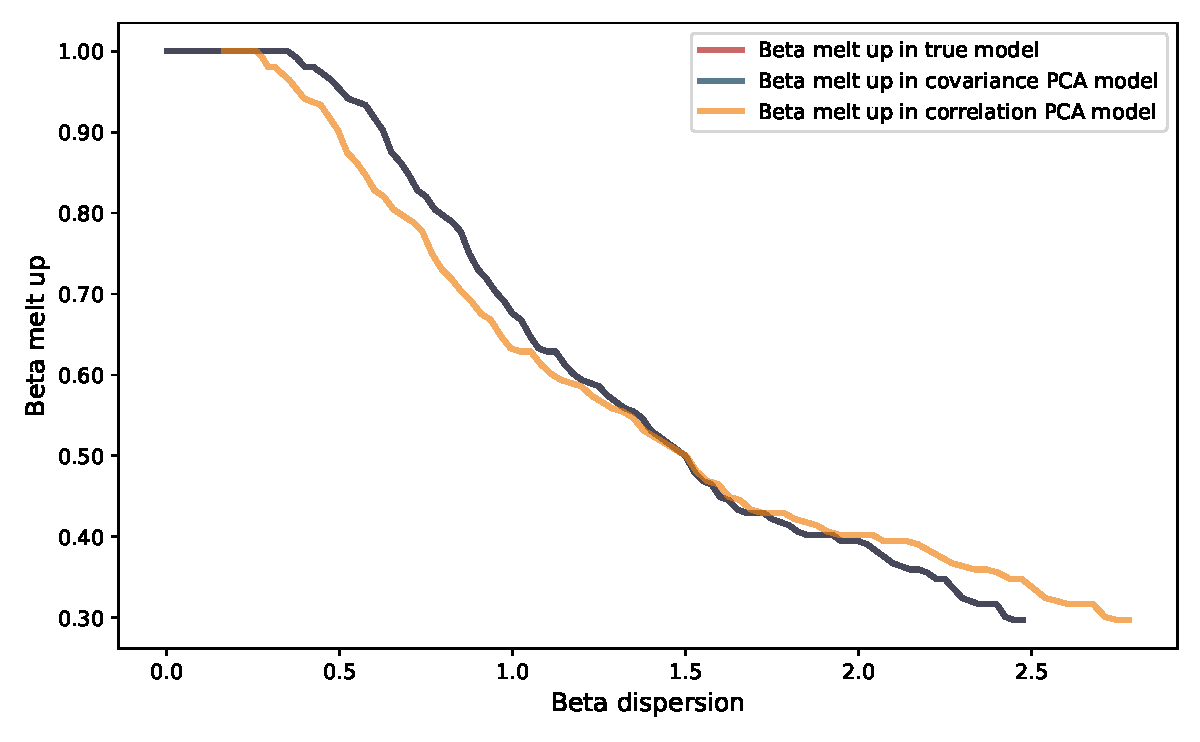
\includegraphics[scale=0.33]{img/DispersionvsMeltup1factorsN512T256fvol25minsvol10maxsvol40}
  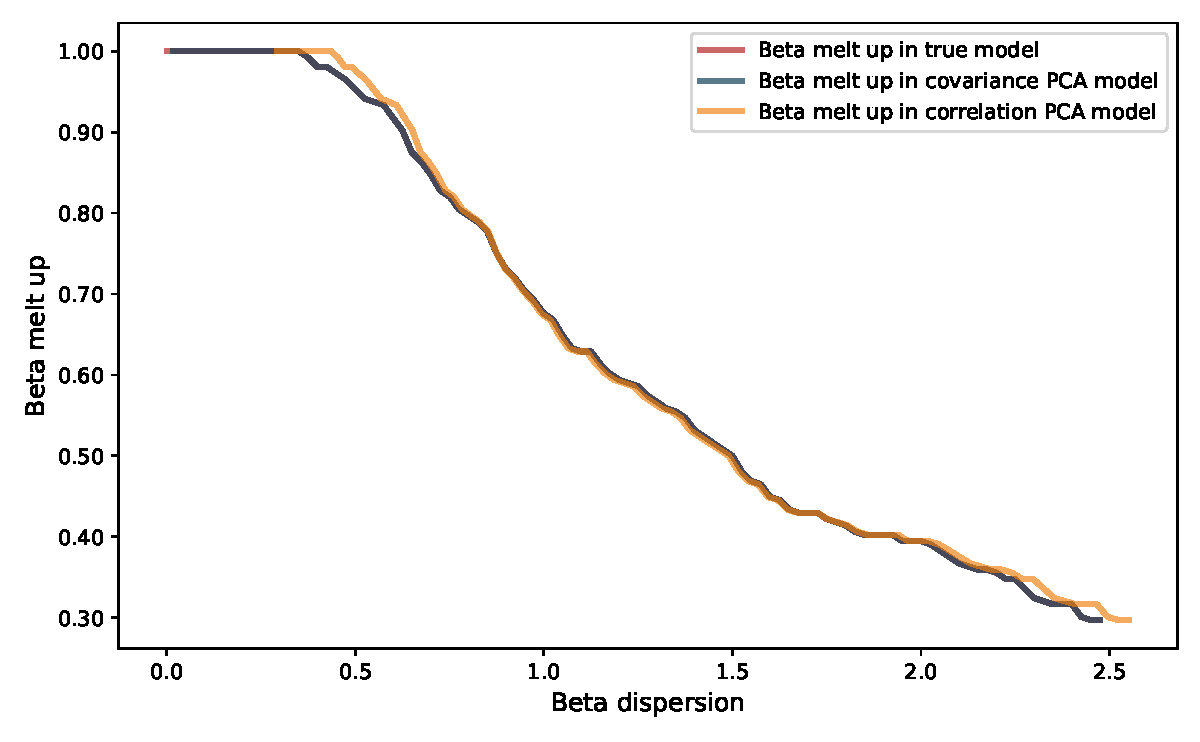
\includegraphics[scale=0.33]{img/DispersionvsMeltup1factorsN512T256fvol16minsvol30maxsvol90}
  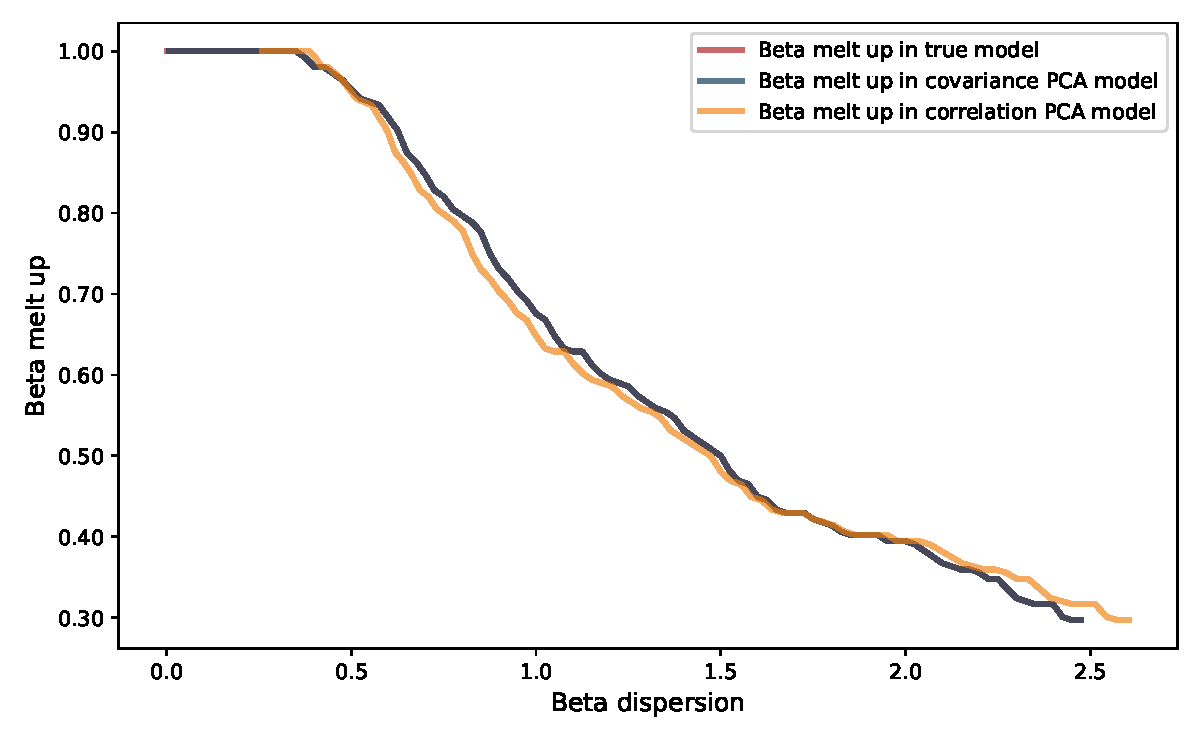
\includegraphics[scale=0.33]{img/DispersionvsMeltup1factorsN512T256fvol25minsvol30maxsvol90}
\end{center}
\caption{Beta dispersion vs Beta Meltup
($p = 512$). 
Top left: $(\sigma_\rmM, \text{ave}(\delta)) = (16,25)$.
Top right: $(\sigma_\rmM, \text{ave}(\delta)) = (25,25)$.
Bottom left: $(\sigma_\rmM, \text{ave}(\delta)) = (16,60)$.
Bottom left: $(\sigma_\rmM, \text{ave}(\delta)) = (25,60)$.
Volatility units are percent annualized.}
\end{figure}




\bibliographystyle{agsm}
\bibliography{biblio}

\end{document}
